\documentclass[
]{jss}

\usepackage[utf8]{inputenc}

\providecommand{\tightlist}{%
  \setlength{\itemsep}{0pt}\setlength{\parskip}{0pt}}

\author{
H. Sherry Zhang\\Monash University \And Dianne Cook\\Monash University
\AND Ursula Laa\\University of Natural Resources and Life Sciences
\AND Nicolas Langrené\\BNU-HKBU United International College
\AND Patricia Menéndez\\Monash University \AND
}
\title{\pkg{cubble}: An R Package for Structuring Spatio-temporal Data}

\Plainauthor{H. Sherry Zhang, Dianne Cook, Ursula Laa, Nicolas
Langrené, Patricia Menéndez}
\Plaintitle{cubble: An R Package for Structuring Spatio-temporal Data}

\Abstract{
Spatio-temporal variables can be divided into time invariant ones that
can be identified by the spatial identifier, or the time varying ones
that cross-identified by the spatial and temporal identifiers. In this
paper, a new data structure, \code{cubble}, is proposed for manipulating
and visualising spatio-temporal data. The new data structure uses two
forms to organise time invariant and varying variables so that the
spatial and temporal dimension of the data can be manipulated separately
while keep synchronised. Advanced considerations are given to illustrate
data with hierarchical structure, data matching, and how cubble fits
with the interactive graphics pipeline. Examples are given to analysing
Australia meteorology data, river level data, and climate reanalysis
(ERA5).
}

\Keywords{spatio temporal, \proglang{R}, climate weather station, data
analysis}
\Plainkeywords{spatio temporal, R, climate weather station, data
analysis}

%% publication information
%% \Volume{50}
%% \Issue{9}
%% \Month{June}
%% \Year{2012}
%% \Submitdate{}
%% \Acceptdate{2012-06-04}

\Address{
    H. Sherry Zhang\\
    Monash University\\
    21 Chancellors Walk, Clayton VIC 3800 Australia\\
  E-mail: \email{huize.zhang@monash.edu}\\
  
      Dianne Cook\\
    Monash University\\
    21 Chancellors Walk, Clayton VIC 3800 Australia\\
  E-mail: \href{mailto:dicook@monash.edu}{\nolinkurl{dicook@monash.edu}}\\
  
      Ursula Laa\\
    University of Natural Resources and Life Sciences\\
    Gregor-Mendel-Straße 33, 1180 Wien, Austria\\
  E-mail: \href{mailto:ursula.laa@boku.ac.at}{\nolinkurl{ursula.laa@boku.ac.at}}\\
  
      Nicolas Langrené\\
    BNU-HKBU United International College\\
    2000 Jintong Road, Tangjiawan, Zhuhai, Guangdong Province, China\\
  E-mail: \href{mailto:nicolas@langrene.com}{\nolinkurl{nicolas@langrene.com}}\\
  
      Patricia Menéndez\\
    Monash University\\
    21 Chancellors Walk, Clayton VIC 3800 Australia\\
  E-mail: \href{mailto:patricia.menendez@monash.edu}{\nolinkurl{patricia.menendez@monash.edu}}\\
  
  }

% Pandoc citation processing

% Pandoc header

\usepackage{amsmath} \usepackage{array} \usepackage{xcolor}

\begin{document}

\newpage

\hypertarget{introduction}{%
\section{Introduction}\label{introduction}}

Spatio-temporal data concerns variables observed in the space across
time and this paper focuses on the spatio-temporal vector data with
fixed locations and regular time interval. This type of data can
naturally been considered as a data cube and here a cube with three
axes: spatial identifier, temporal identifier, and variable can be used
to conceptualise spatio-temporal data. In this cubic formation, space
only occupy one dimension, rather than two, to avoid the needs of
hypercube for multivariate spatio-temporal data.

While conceptually the data format is relatively simple, the actual data
object that comes to the analysts in the analysis can be in various
forms. Figure \ref{fig:illu-input} shows four examples of wild
spatio-temporal data: 1) combines the time invariant and varying
variables into a single table through duplicating the time invariant
variables; 2) splits those variables into a separate spatial table and a
temporal table; 3) \ldots; and lastly 4) is array-based data, like
NetCDF (Network Common Data Form) data, which is commonly used in earth
science, e.g.~climatology, meteorology, and oceanography, among others,
to organise multivariate data in a spatio-temporal grid.

\begin{CodeChunk}
\begin{figure}

{\centering 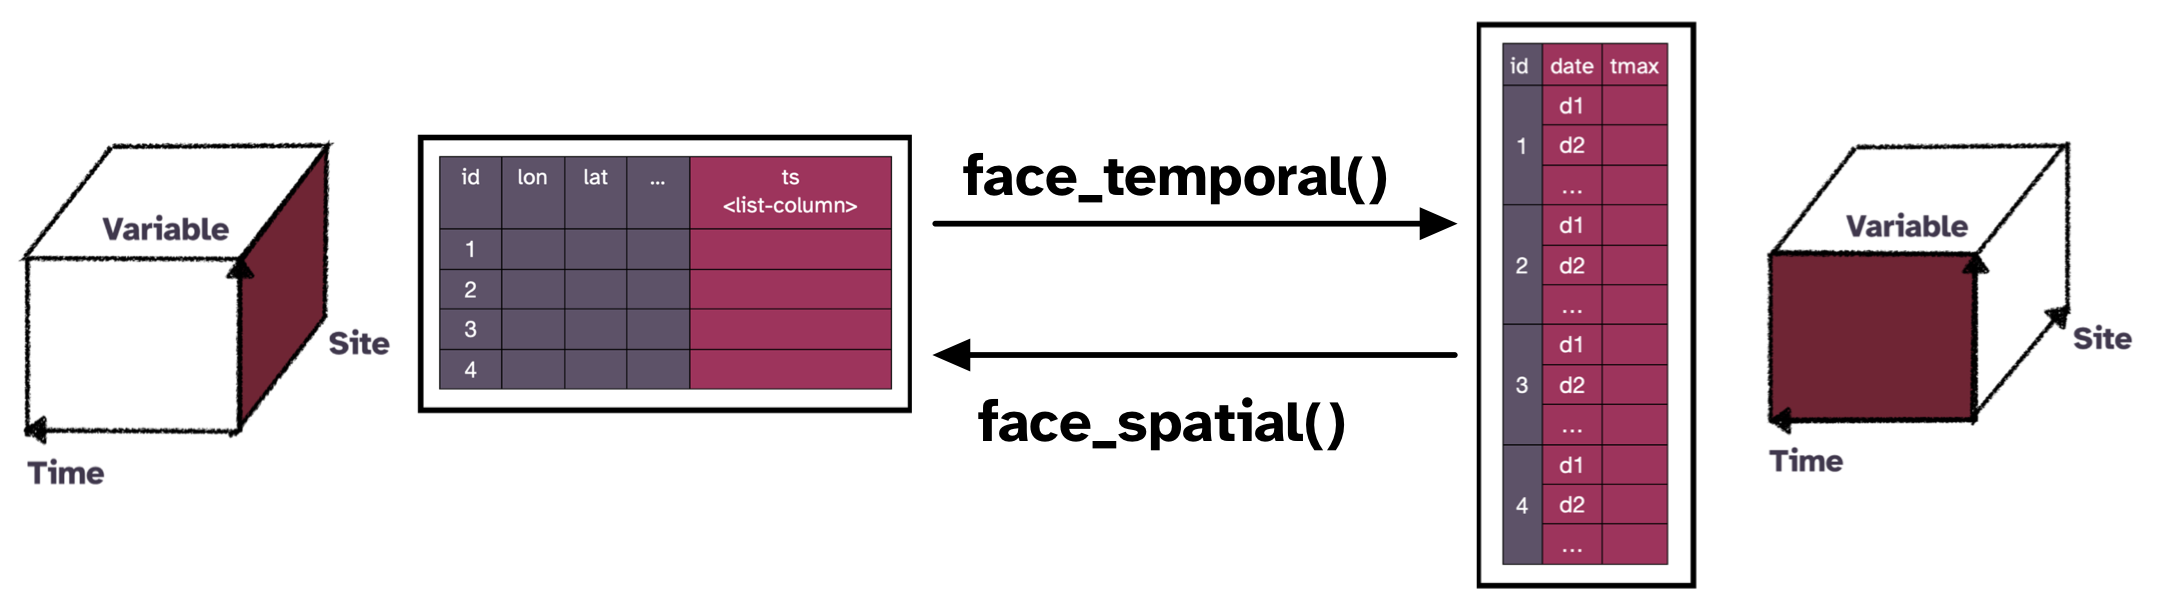
\includegraphics[width=1\linewidth,height=0.4\textheight]{/Users/sherryzhang/Documents/research/paper-cubble/figures/diagram-keynotes/diagram-keynotes.001} 

}

\caption[An illustration of different spatio-temporal data format]{An illustration of different spatio-temporal data format: (1) a single table for all the variables; (2) separate tables for spatial and temporal variables; (3) a table of metadata used to query the database and a separate table for queried data; and (4) an array data structure.}\label{fig:illu-input}
\end{figure}
\end{CodeChunk}

Different authors have proposed various data objects to work with
spatial temporal data in \proglang{R} and this includes: \pkg{spacetime}
\citep{spacetime} is built on the \pkg{sp} \citep{sp} and \pkg{xts}
\citep{xts} class and both of which have been replaced by more recent
spatial and temporal data objects. \pkg{spatstat} \citep{spatstat}
implements a \texttt{ppp} class for analysing point pattern data; and
more recent, \pkg{stars} \citep{stars} has implemented an
spatio-temporal array for wrangling both vector and raster data.

\textcolor{red}{Think again on the motivation and why it is hard to work existing tools.}
In spatio-temporal data analysis, analysts will receive one of the
various data formats depends on the data provider and need to manually
rearrange the data to fit into one of the data object in \proglang{R}
before starting any analysis on the data itself.

Looking at spatial or temporal data analysis, data objects like \pkg{sf}
\citep{sf} and \pkg{tsibble} \citep{tsibble} have smoothed the data
analysis in these two domains while there has not yet been a
spatio-temporal data structure that makes it easy to explore
spatio-temporal data and this creates a gap in the software development.
The requirement for such a tool is important given the ubiquity of
spatio-temporal vector data in the wild: climate observations from
weather stations, air quality variables from air monitoring stations, or
any variables that are measured at fixed location across time.

This paper describes the implementation of a new spatio-temporal data
structure: \pkg{cubble}. \pkg{Cubble} implements a data structure that
uses two forms to manage the switch between spatial and temporal
dimension. With this structure, users can manipulate the spatial or
temporal dimension separately, while leaves the linking of two
dimensions to \pkg{cubble}. The software is available from the
Comprehensive R Archive Network (CRAN) at {[}CRAN link{]}.

The rest of the paper is divided as follows: Section 2 presents the
workflow of data manipulation in cubble. Section 3 explains how cubble
deals with some advanced considerations including data with hierarchical
structure, data matching, and how cubble fits with existing static and
interactive visualisation tools. Section 4 gives examples of the
features introduced in the previous two sections with climate and
hydrology data. An example on how cubble handle NetCDF data is also
provided. Section 5 concludes the paper.

\hypertarget{the-cubble-package}{%
\section{The cubble package}\label{the-cubble-package}}

This section will present two formats that cubble uses to arrange
spatio-temporal data. Main cubble functions will then be introduced to
illustrate how to work with these two formats in short examples. Lastly,
a subsection will dedicate to how existing packages, in spatial and
temporal analysis, fit in with cubble.

In cubble, data can represented in two formats: nested form and long
form, and Figure \ref{fig:illu-cubble} sketches the two forms with the
associated attributes. The decision on which form to use in data
manipulation is output-oriented, meaning analysts need to first think
about whether the output of an operation is identified only by the
spatial identifier, or a combination of spatial and temporal identifier.
The nested cubble is suitable for working with operations that are only
identified by the site and this type of operation can be a pure
manipulation of time invariant variables, or an operation that
summarises time varying variables into site. Underneath the nested form,
a cubble is built from a \code{rowwise_df} class where each site forms a
separate group. This structure simplifies the calculation that involves
temporal variables by avoiding the use of \code{purrr::map()} syntax
when working with list-column.

For those operations whose output involves both a spatial and temporal
identifier, long form should be used. The long form uses a
\code{grouped_df} class to forms all the time of a site as a group. Time
invariant variables are stored separately as an special attribute of the
long cubble. This design avoids repeating the spatial variables at each
time stamp while not dropping information from spatial variables.

\begin{CodeChunk}
\begin{figure}

{\centering 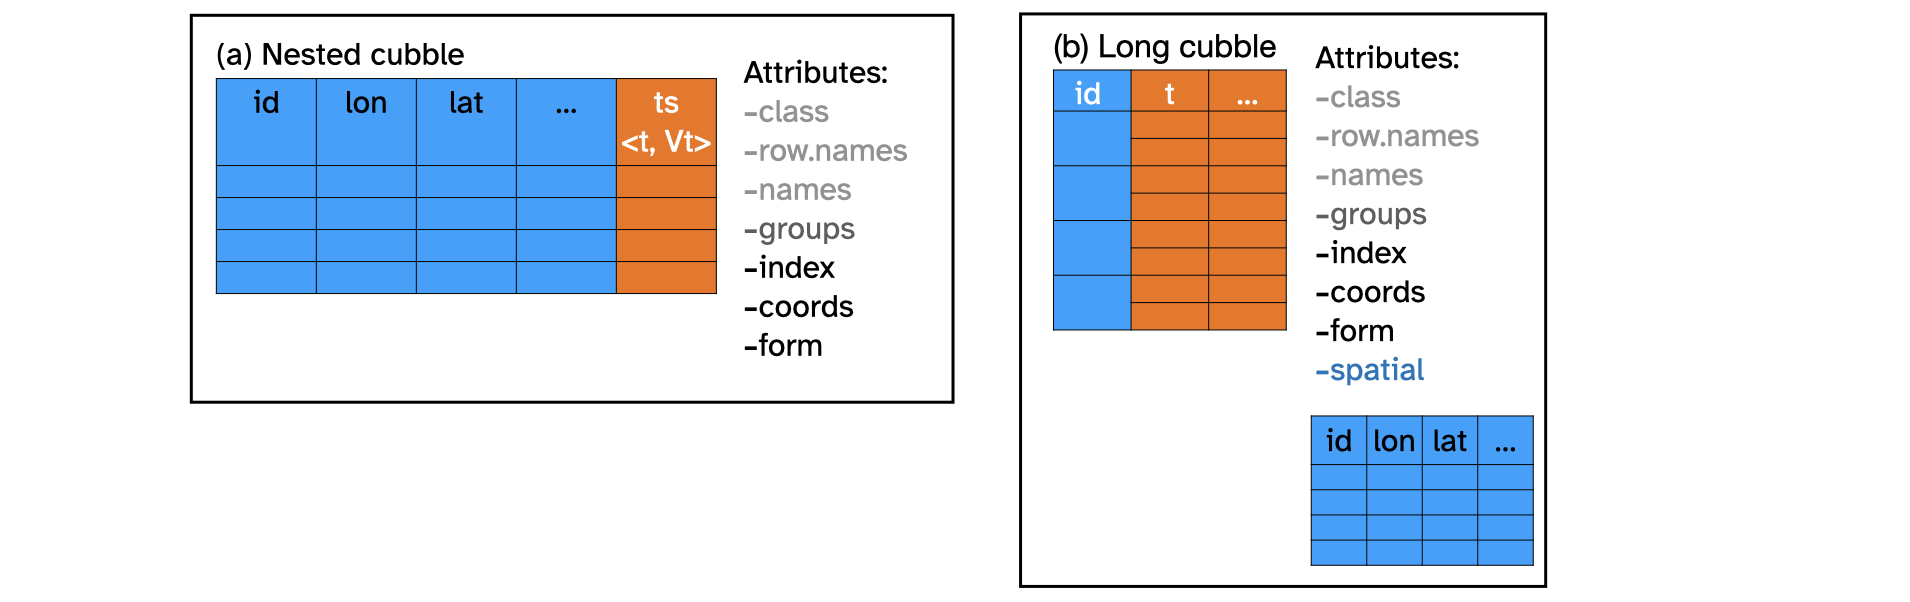
\includegraphics[width=1\linewidth]{/Users/sherryzhang/Documents/research/paper-cubble/figures/diagram-keynotes/diagram-keynotes.002} 

}

\caption{An illustration of the nested and long form in cubble. The nested form defines each site in a row and nests the time varying variables into a single column \code{ts}. The long form cubble uses \code{id} and \code{t} to identify each row and store the time invariant variables as an attribute, \code{spatial}.}\label{fig:illu-cubble}
\end{figure}
\end{CodeChunk}

\hypertarget{create-a-cubble-in-the-nested-form}{%
\subsection{Create a cubble in the nested
form}\label{create-a-cubble-in-the-nested-form}}

To use functions in the \texttt{cubble} package, an analyst will first
need to turn the data object into a \code{cubble} class.
\code{as_cubble()} does this through supplying the three key components:
\code{key} as the spatial identifier; \code{index} as the temporal
identifier; and a vector of \code{coords} in the order of longitude and
latitude. The use of \code{key} and \code{index} follows the design in
the \pkg{tsibble} package and the cubble created by default is in the
nested form.

Before the formal examples in Section \ref{examples}, each function
introduced in this section will be accompanied by a small example. The
data used for the small examples is a subset of a larger climate weather
station data used in the formal examples and has been simplified to
include only five weather stations. It contains spatial information of
each station: station id, latitude, longitude, elevation, station name
and World Meteorology Organisation ID and also daily temporal
information of date, maximum and minimum temperature and precipitation
for 2020. \code{climate_flat} stores this data in format 1) in Figure
\ref{fig:illu-input} and the code below creates a cubble out of
\code{climate_flat} with \code{id} as the key, \code{date} as the index,
and \code{c(long, lat)} as the coordinates:

\begin{CodeChunk}
\begin{CodeInput}
R> cubble_nested <- cubble::climate_flat %>%
+   as_cubble(key = id, index = date, coords = c(long, lat))
R> cubble_nested
\end{CodeInput}
\begin{CodeOutput}
# cubble:   id [5]: nested form
# bbox:     [115.97, -32.94, 133.55, -12.42]
# temporal: date [date], prcp [dbl], tmax [dbl], tmin [dbl]
  id            lat  long  elev name           wmo_id ts                
  <chr>       <dbl> <dbl> <dbl> <chr>           <dbl> <list>            
1 ASN00009021 -31.9  116.  15.4 perth airport   94610 <tibble [366 x 4]>
2 ASN00010311 -31.9  117. 179   york            94623 <tibble [366 x 4]>
3 ASN00010614 -32.9  117. 338   narrogin        94627 <tibble [366 x 4]>
4 ASN00014015 -12.4  131.  30.4 darwin airport  94120 <tibble [366 x 4]>
5 ASN00015131 -17.6  134. 220   elliott         94236 <tibble [366 x 4]>
\end{CodeOutput}
\end{CodeChunk}

There are a few information in the cubble header: the name of the
\code{key} variable: \code{id} and its unique number: 5, the bounding
box: \code{[115.97, -32.94, 133.55, -12.42]} , and also the name of
variable nested in the \code{ts} column with its type:
\code{date [date], prcp [dbl], tmax [dbl], tmin [dbl]}.

\hypertarget{stretch-a-nested-cubble-into-the-long-form}{%
\subsection{Stretch a nested cubble into the long
form}\label{stretch-a-nested-cubble-into-the-long-form}}

The nested format is convenient for those operations whose output
doesn't contain a time dimension, for those outputs that are
cross-identified by the spatial and temporal identifier, a long cubble
needs to be used. The function \code{stretch()} is designed to switch
the cubble from the nested form to the long form. This code shows how to
switch the nested cubble just created into its long form:

\begin{CodeChunk}
\begin{CodeInput}
R> cubble_long <- cubble_nested %>% stretch()
R> cubble_long
\end{CodeInput}
\begin{CodeOutput}
# cubble:  date, id [5]: long form
# bbox:    [115.97, -32.94, 133.55, -12.42]
# spatial: lat [dbl], long [dbl], elev [dbl], name [chr], wmo_id [dbl]
  id          date        prcp  tmax  tmin
  <chr>       <date>     <dbl> <dbl> <dbl>
1 ASN00009021 2020-01-01     0  31.9  15.3
2 ASN00009021 2020-01-02     0  24.9  16.4
3 ASN00009021 2020-01-03     6  23.2  13  
4 ASN00009021 2020-01-04     0  28.4  12.4
5 ASN00009021 2020-01-05     0  35.3  11.6
# ... with 1,825 more rows
\end{CodeOutput}
\end{CodeChunk}

Notice that the third line in the header now shows the name and type of
spatial variables:
\code{lat [dbl], long [dbl], elev [dbl], name [chr], wmo_id [dbl]} and
these variables are now stored as a \code{spatial} attribute of the
data:

\begin{CodeChunk}
\begin{CodeInput}
R> attr(cubble_long, "spatial")
\end{CodeInput}
\begin{CodeOutput}
# A tibble: 5 x 6
  id            lat  long  elev name           wmo_id
  <chr>       <dbl> <dbl> <dbl> <chr>           <dbl>
1 ASN00009021 -31.9  116.  15.4 perth airport   94610
2 ASN00010311 -31.9  117. 179   york            94623
3 ASN00010614 -32.9  117. 338   narrogin        94627
4 ASN00014015 -12.4  131.  30.4 darwin airport  94120
5 ASN00015131 -17.6  134. 220   elliott         94236
\end{CodeOutput}
\end{CodeChunk}

\hypertarget{tamp-a-long-cubble-back-to-the-nested-form}{%
\subsection{Tamp a long cubble back to the nested
form}\label{tamp-a-long-cubble-back-to-the-nested-form}}

Manipulation on the spatial and temporal dimension can be an iterative
process and analysts may need to go back and forth between the nested
and long cubble. \code{tamp()}, an inverse of \code{stretch()}, switches
a long cubble to a nested cubble:

\begin{CodeChunk}
\begin{CodeInput}
R> cubble_back <- cubble_long %>% tamp()
R> cubble_back
\end{CodeInput}
\begin{CodeOutput}
# cubble:   id [5]: nested form
# bbox:     [115.97, -32.94, 133.55, -12.42]
# temporal: date [date], prcp [dbl], tmax [dbl], tmin [dbl]
  id            lat  long  elev name           wmo_id ts                
  <chr>       <dbl> <dbl> <dbl> <chr>           <dbl> <list>            
1 ASN00009021 -31.9  116.  15.4 perth airport   94610 <tibble [366 x 4]>
2 ASN00010311 -31.9  117. 179   york            94623 <tibble [366 x 4]>
3 ASN00010614 -32.9  117. 338   narrogin        94627 <tibble [366 x 4]>
4 ASN00014015 -12.4  131.  30.4 darwin airport  94120 <tibble [366 x 4]>
5 ASN00015131 -17.6  134. 220   elliott         94236 <tibble [366 x 4]>
\end{CodeOutput}
\end{CodeChunk}

\hypertarget{migrate-spatial-variables-to-a-long-cubble}{%
\subsection{Migrate spatial variables to a long
cubble}\label{migrate-spatial-variables-to-a-long-cubble}}

Sometimes, analysts may need to apply some variable transformation that
involves both the spatial and temporal variable. An example of this is
the transformation of temporal variables into the spatial dimension in
glyph maps(which will be elaborated in section \ref{st_transformation}).
Cubble allows this operation through \code{migrate()}, which moves the
specified spatial variables into the long cubble:

\begin{CodeChunk}
\begin{CodeInput}
R> cubble_mig <- cubble_long %>% migrate(long, lat)
R> cubble_mig
\end{CodeInput}
\begin{CodeOutput}
# cubble:  date, id [5]: long form
# bbox:    [115.97, -32.94, 133.55, -12.42]
# spatial: lat [dbl], long [dbl], elev [dbl], name [chr], wmo_id [dbl]
  id          date        prcp  tmax  tmin  long   lat
  <chr>       <date>     <dbl> <dbl> <dbl> <dbl> <dbl>
1 ASN00009021 2020-01-01     0  31.9  15.3  116. -31.9
2 ASN00009021 2020-01-02     0  24.9  16.4  116. -31.9
3 ASN00009021 2020-01-03     6  23.2  13    116. -31.9
4 ASN00009021 2020-01-04     0  28.4  12.4  116. -31.9
5 ASN00009021 2020-01-05     0  35.3  11.6  116. -31.9
# ... with 1,825 more rows
\end{CodeOutput}
\end{CodeChunk}

This function should generally be used in the last step of the analysis
since it is a temporary operation, meaning these added spatial variables
are not stored in the long form and will disappear if switched to the
nested form and then switched back:

\begin{CodeChunk}
\begin{CodeInput}
R> cubble_mig %>% tamp() %>% stretch()
\end{CodeInput}
\begin{CodeOutput}
# cubble:  date, id [5]: long form
# bbox:    [115.97, -32.94, 133.55, -12.42]
# spatial: long [dbl], lat [dbl], elev [dbl], name [chr], wmo_id [dbl]
  id          date        prcp  tmax  tmin
  <chr>       <date>     <dbl> <dbl> <dbl>
1 ASN00009021 2020-01-01     0  31.9  15.3
2 ASN00009021 2020-01-02     0  24.9  16.4
3 ASN00009021 2020-01-03     6  23.2  13  
4 ASN00009021 2020-01-04     0  28.4  12.4
5 ASN00009021 2020-01-05     0  35.3  11.6
# ... with 1,825 more rows
\end{CodeOutput}
\end{CodeChunk}

\hypertarget{compatibility-with-existing-packages}{%
\subsection{Compatibility with existing
packages}\label{compatibility-with-existing-packages}}

The previous four subsections have introduced operations specific to the
\code{cubble} class and this section will demonstrate how the
\code{cubble} class interacts with existing packages commonly used in
spatial and temporal analysis, specifically, \code{dplyr},
\code{tsibble}, \code{sf} (\code{s2}), and \code{netcdf4}.

\hypertarget{dplyr}{%
\subsubsection{dplyr}\label{dplyr}}

The \code{dplyr} package has provided many tools for data wrangling
tasks and these operations are useful in the spatio-temporal context.
\code{cubble} provides methods that support the following \code{dplyr}
verbs in both the nested and long form:

\begin{quote}
\texttt{mutate}, \texttt{filter}, \texttt{summarise}, \texttt{select},
\texttt{arrange}, \texttt{rename}, \texttt{left\_join}, and the slice
family (\texttt{slice\_head}, \texttt{slice\_tail},
\texttt{slice\_sample}, \texttt{slice\_min}, \texttt{slice\_max})
\end{quote}

\textcolor{red}{more work on groupby} The grouping pair, \code{group_by}
and \code{ungroup}, can only be used in the long form to define grouping
on the time but not in the nested form.

\hypertarget{tsibble}{%
\subsubsection{tsibble}\label{tsibble}}

\code{tsibble} is a temporal data structure that uses \code{index} and
\code{key} to identify the time and different series and \code{cubble}
can be seen as a natural extension of \code{tsibble} for spatio-temporal
data with an additional coordinates component and using two forms to
arrange variables. This makes it easy to cast a \code{tsibble} into a
\code{cubble} as only the \code{coords} argument needs to be supplied:

\begin{CodeChunk}
\begin{CodeInput}
R> # demonstrate with a tsibble created from climate_flat
R> raw <- climate_flat %>% 
+   tsibble::as_tsibble(key = id, index = date) 
R> 
R> dt <-  raw %>% 
+   cubble::as_cubble(coords = c(long, lat))
R> dt
\end{CodeInput}
\begin{CodeOutput}
# cubble:   id [5]: nested form
# bbox:     [115.97, -32.94, 133.55, -12.42]
# temporal: date [date], prcp [dbl], tmax [dbl], tmin [dbl]
  id            lat  long  elev name           wmo_id ts                
  <chr>       <dbl> <dbl> <dbl> <chr>           <dbl> <list>            
1 ASN00009021 -31.9  116.  15.4 perth airport   94610 <tbl_ts [366 x 4]>
2 ASN00010311 -31.9  117. 179   york            94623 <tbl_ts [366 x 4]>
3 ASN00010614 -32.9  117. 338   narrogin        94627 <tbl_ts [366 x 4]>
4 ASN00014015 -12.4  131.  30.4 darwin airport  94120 <tbl_ts [366 x 4]>
5 ASN00015131 -17.6  134. 220   elliott         94236 <tbl_ts [366 x 4]>
\end{CodeOutput}
\end{CodeChunk}

In the nested cubble created, each element in the list-column \code{ts}
is of \code{tbl_ts} class and operations available to the tsibble class
is still valid under cubble. For example, the code below calculates two
features of the maximum temperature:

\begin{CodeChunk}
\begin{CodeInput}
R> # add station-based features in the nested form.
R> dt %>% 
+   mutate(fabletools::features(ts, tmax, list(tmax_mean = mean, tmax_var = var)))
\end{CodeInput}
\begin{CodeOutput}
# cubble:   id [5]: nested form
# bbox:     [115.97, -32.94, 133.55, -12.42]
# temporal: date [date], prcp [dbl], tmax [dbl], tmin [dbl]
  id            lat  long  elev name           wmo_id ts      tmax_mean tmax_var
  <chr>       <dbl> <dbl> <dbl> <chr>           <dbl> <list>      <dbl>    <dbl>
1 ASN00009021 -31.9  116.  15.4 perth airport   94610 <tbl_t~      25.7    38.6 
2 ASN00010311 -31.9  117. 179   york            94623 <tbl_t~      26.2    51.1 
3 ASN00010614 -32.9  117. 338   narrogin        94627 <tbl_t~      23.7    45.4 
4 ASN00014015 -12.4  131.  30.4 darwin airport  94120 <tbl_t~      33.1     3.02
5 ASN00015131 -17.6  134. 220   elliott         94236 <tbl_t~      34.6    24.7 
\end{CodeOutput}
\end{CodeChunk}

\hypertarget{sf-and-s2}{%
\subsubsection{sf and s2}\label{sf-and-s2}}

As a spatial data object, \code{sf} creates a simple feature geometry
list-column (\code{sfc}) in the data frame to provide spatial operations
on various geometry types (\code{POINT}, \code{LINESTRING},
\code{POLYGON}, \code{MULTIPOLYGON}, etc). These spatial operations are
also valuable for spatio-temporal data analysis, but an \code{sf} object
\emph{usually} don't contain temporal variables. This means \code{sf}
can't be directly cast into a \code{cubble}, however, \code{cubble} does
support \code{sfc} columns in the nested form and spatial operations
applied to the \code{sfc} column in \code{sf} can still be applied to
the \code{sfc} column in a cubble. The following example shows how to
create an \code{sfc} column of \code{POINT} type from latitude and
longitude in cubble. Then \code{sf::st_within} is used to add the state
\code{MULTIPOLYGON} of each weather station before a coordinate
transformation is made.

\begin{CodeChunk}
\begin{CodeInput}
R> library(sf)
R> # create a cubble
R> cb <- climate_flat %>% 
+   cubble::as_cubble(key = id, index = date, coords = c(long, lat))
R> 
R> aus <- ozmaps::abs_ste
R> 
R> dt <- cb %>%
+   mutate(
+     # create `sfc` column based on long and lat
+     ll = st_sfc(
+       purrr::map2(long, lat, ~st_point(c(.x, .y))),
+       crs = st_crs(aus)),
+     
+     # append state multi-polygon based on the `sfc` created
+     state = aus$geometry[st_within(ll, aus, sparse = FALSE)],
+     
+     # adopt a different projection: lambert conformal conic (EPSG:3112)
+     state = st_transform(state, crs = "EPSG:3112")
+     )
R> 
R> dt
\end{CodeInput}
\begin{CodeOutput}
# cubble:   id [5]: nested form
# bbox:     [115.97, -32.94, 133.55, -12.42]
# temporal: date [date], prcp [dbl], tmax [dbl], tmin [dbl]
  id            lat  long  elev name         wmo_id ts                        ll
  <chr>       <dbl> <dbl> <dbl> <chr>         <dbl> <list>           <POINT [°]>
1 ASN00009021 -31.9  116.  15.4 perth airpo~  94610 <tibble~ (115.9764 -31.9275)
2 ASN00010311 -31.9  117. 179   york          94623 <tibble~  (116.765 -31.8997)
3 ASN00010614 -32.9  117. 338   narrogin      94627 <tibble~ (117.1797 -32.9342)
4 ASN00014015 -12.4  131.  30.4 darwin airp~  94120 <tibble~ (130.8925 -12.4239)
5 ASN00015131 -17.6  134. 220   elliott       94236 <tibble~ (133.5407 -17.5521)
# ... with 1 more variable: state <MULTIPOLYGON [m]>
\end{CodeOutput}
\end{CodeChunk}

An \pkg{s2} \code{lnglat} vector can similarly be created as an
\code{sfc} in cubble before using any \code{s2}-prefixed function:

\begin{CodeChunk}
\begin{CodeInput}
R> library(s2)
R> # western australia map
R> wa <- ozmaps::abs_ste %>% filter(NAME == "Western Australia")
R> 
R> # mutate a `s2_lnglat` vector on `cb` created in the last chunk
R> cb %>%
+   mutate(ll = s2_lnglat(long, lat)) %>% 
+   filter(s2_within(ll, wa))
\end{CodeInput}
\begin{CodeOutput}
# cubble:   id [3]: nested form
# bbox:     [115.97, -32.94, 117.18, -31.89]
# temporal: date [date], prcp [dbl], tmax [dbl], tmin [dbl]
  id            lat  long  elev name          wmo_id ts                 ll      
  <chr>       <dbl> <dbl> <dbl> <chr>          <dbl> <list>             <s2_lng>
1 ASN00009021 -31.9  116.  15.4 perth airport  94610 <tibble [366 x 4]> (115.97~
2 ASN00010311 -31.9  117. 179   york           94623 <tibble [366 x 4]> (116.76~
3 ASN00010614 -32.9  117. 338   narrogin       94627 <tibble [366 x 4]> (117.17~
\end{CodeOutput}
\end{CodeChunk}

\hypertarget{netcdf}{%
\subsubsection{netcdf}\label{netcdf}}

NetCDF data has two main components: \emph{dimension} for defining the
spatio-temporal grid (longitude, latitude, and time) and \emph{variable}
that populates the defined grid. Attributes are usually associated with
dimension and variable in the NetCDF format data and a
\href{http://cfconventions.org/}{metadata convention for climate and
forecast} has been designed to standardise the format of the attributes.
A few packages in R exists for manipulating NetCDF data and this
includes a high-level R interface: \pkg{ncdf4} \citep{ncdf4}, a
low-level interface that calls C-interface: \pkg{RNetCDF}
\citep{rnetcdf, michna2013rnetcdf}, and a tidyverse implementation:
\pkg{tidync} \citep{tidync}.

Cubble provides an \code{as_cubble()} method to coerce the \code{ncdf4}
class from the \pkg{ncdf4} package into a \code{cubble}. It maps each
combination of longitude and latitude into an \code{id} as the
\code{key}:

\begin{CodeChunk}
\begin{CodeInput}
R> # read in the .nc file as a ncdf4 class
R> raw <- ncdf4::nc_open(here::here("data/era5-pressure.nc"))
R> 
R> # convert the variable q and z in the ncdf4 into a cubble
R> dt <- as_cubble(raw, vars = c("q", "z"))
\end{CodeInput}
\end{CodeChunk}

Memory limit with NetCDF data in cubble depends on longitude grid point
x latitude grid point x time grid point x number of variable. Cubble can
handle slightly more than 300 x 300 (longitude x longitude) grid points
for 3 variables in one year and spatial grid can be reduced to trade for
longer time period and more variables. A 300 by 300 spatial grid can be
a bounding box of {[}100, -80, 180, 0{]} at 0.25 degree resolution or a
global bounding box {[}-180, -90, 180, -90{]} at 1 degree resolution.
Subsetting longitude and latitude grid is available through
\code{long_range} and \code{lat_range} if the NetCDF file has finer
resolution than needed.

\begin{CodeChunk}
\begin{CodeInput}
R> # Assume my_ncdf has bounding box of [-180, -90, 180, -90] 
R> # at 0.25 degree resolution and subset it to have 
R> # 1 degree resolution:
R> dt <- as_cubble(my_ncdf, vars = c("q", "z"), 
+                 long_range = seq(-180, 180, 1), 
+                 lat_range = seq(-90, 90, 1))
\end{CodeInput}
\end{CodeChunk}

\hypertarget{other-features-and-considerations}{%
\section{Other features and
considerations}\label{other-features-and-considerations}}

\hypertarget{hierarchical-structure}{%
\subsection{Hierarchical structure}\label{hierarchical-structure}}

Spatial locations can have grouping structure either inherent to the
data or formed by clustering. Rather than analysing variables in the
site level, summarised variables in the cluster level can give a crisper
picture of local areas. In cubble, \code{switch_key()} can be used to
create a new level of grouping of spatial locations by specifying a
clustering variable. Figure \ref{fig:illu-hier} illustrates the
relationship of cubbles at station and cluster level, in both the long
and nested form. By specifying
\code{cluster_nested <- station_nested \%>\% switch_key(key = cluster)},
the cubble re-defines the cubble key from \code{id} in
\code{station_nested} to \code{cluster} in \code{cluster_nested}. All
the spatial variables variant to \code{cluster} are now nested into a
\code{.val} column and cluster level variables can be computed in the
same fashion as station level variables in \code{station_nested}.

\begin{CodeChunk}
\begin{figure}

{\centering 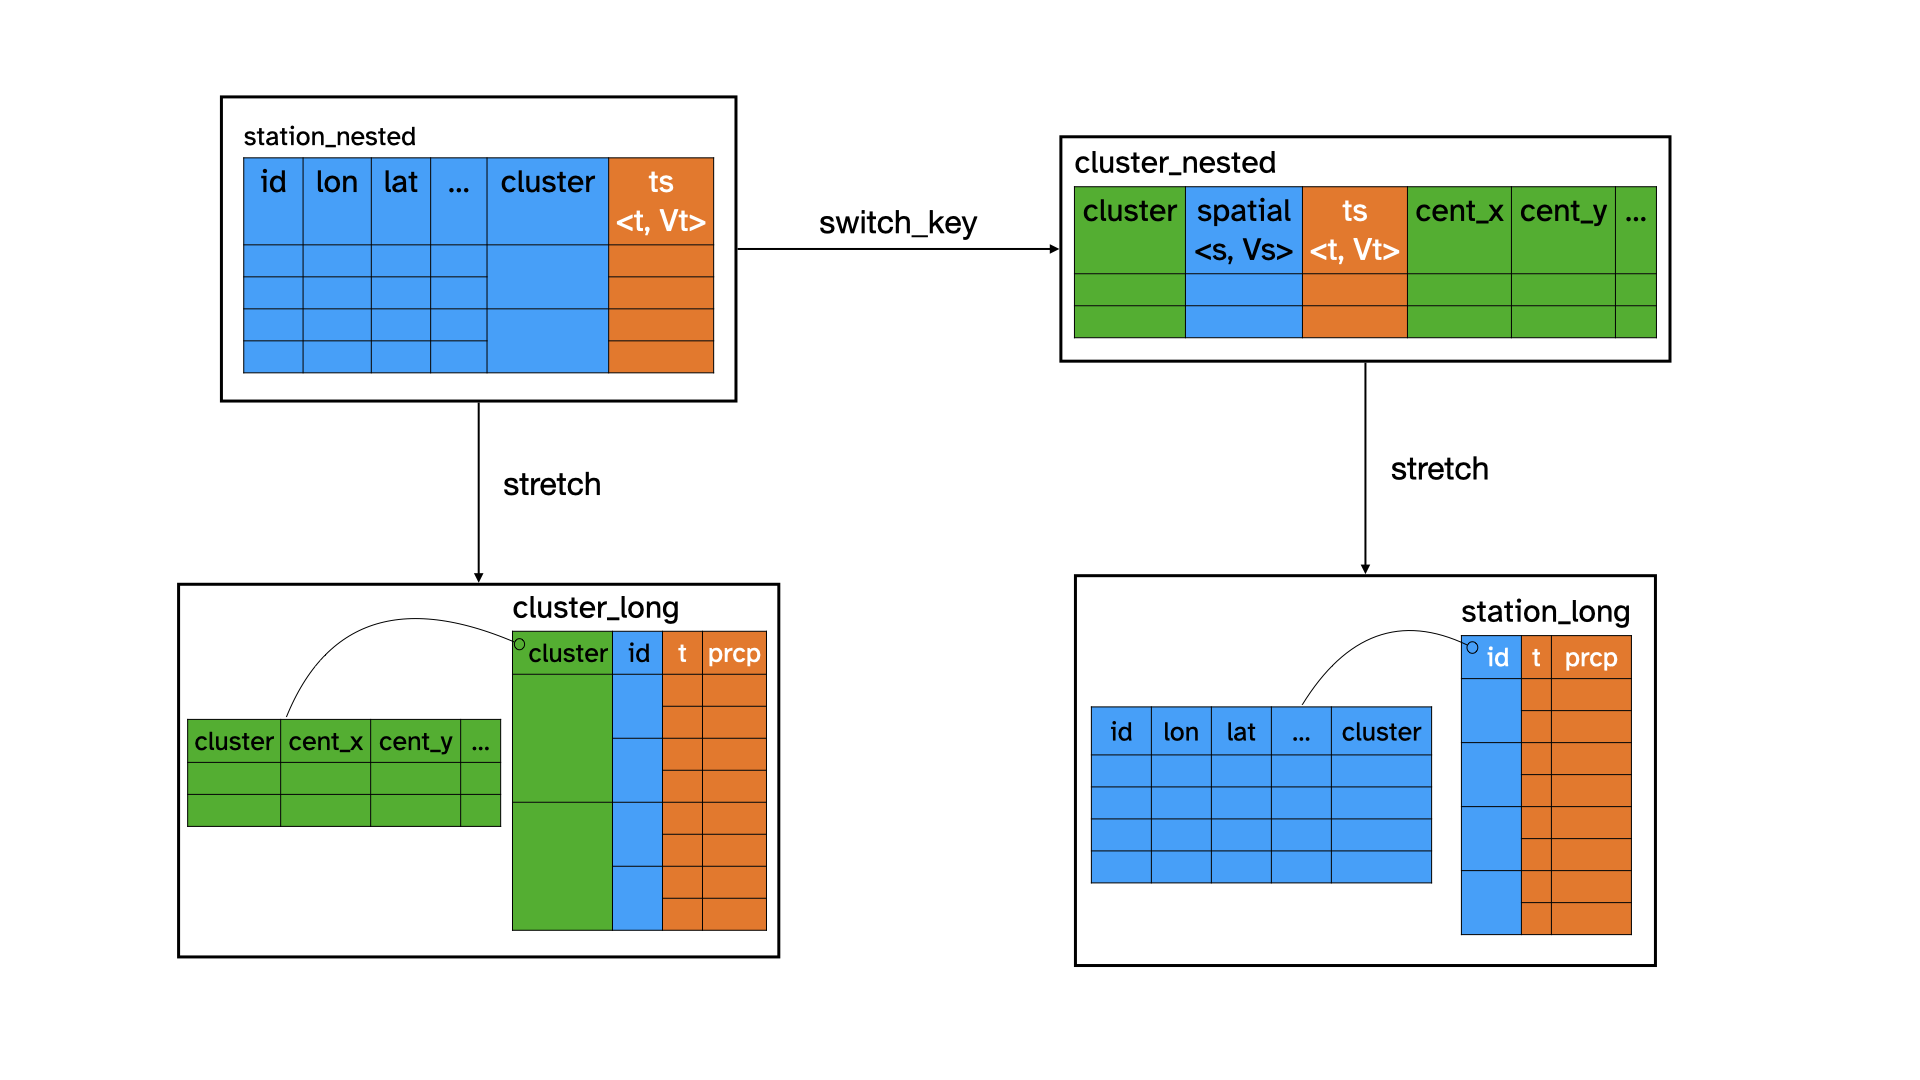
\includegraphics[width=1\linewidth,height=0.4\textheight]{/Users/sherryzhang/Documents/research/paper-cubble/figures/diagram-keynotes/diagram-keynotes.003} 

}

\caption[An illustration of the original and cluster level cubble in the nested form long form for hierarchical structure data]{An illustration of the original and cluster level cubble in the nested form long form for hierarchical structure data. \code{switch\_key()} changes the station level cubble into a cluster level cubble and both can be stretched into the long form.}\label{fig:illu-hier}
\end{figure}
\end{CodeChunk}

\hypertarget{data-fusion-and-matching}{%
\subsection{Data fusion and matching}\label{data-fusion-and-matching}}

\textcolor{red}{more beginning} Cubble provides functionality for
matching sites from two data sources. To be a valid pair of matching,
the matched pair from different data sources need to:

\begin{itemize}
\tightlist
\item
  be spatially close to each other, and
\item
  have similar temporal movement
\end{itemize}

\code{match_sites()} matches data based on these two criteria: it first
matches the two data sources spatially through computing the pairwise
distance on latitude and longitude. Pairs that pass the spatial matching
are then matched temporally through computing the number of matched
peaks within a fixed length window. Figure \ref{fig:illu-matching}
illustrates this temporal matching in more details. Given two series
\code{A} and \code{a}, 3 peaks have been picked in each series. An
interval, with default length of 5, is constructed for each peak in
series \code{A} and the peaks in series \code{a} are tested against
whether they fall into the any of the intervals. In this illustration,
there are 2 matches for these two series. Several arguments are
available in \code{match_sites()} to fine-tune the matching:

\begin{CodeChunk}
\begin{figure}

{\centering 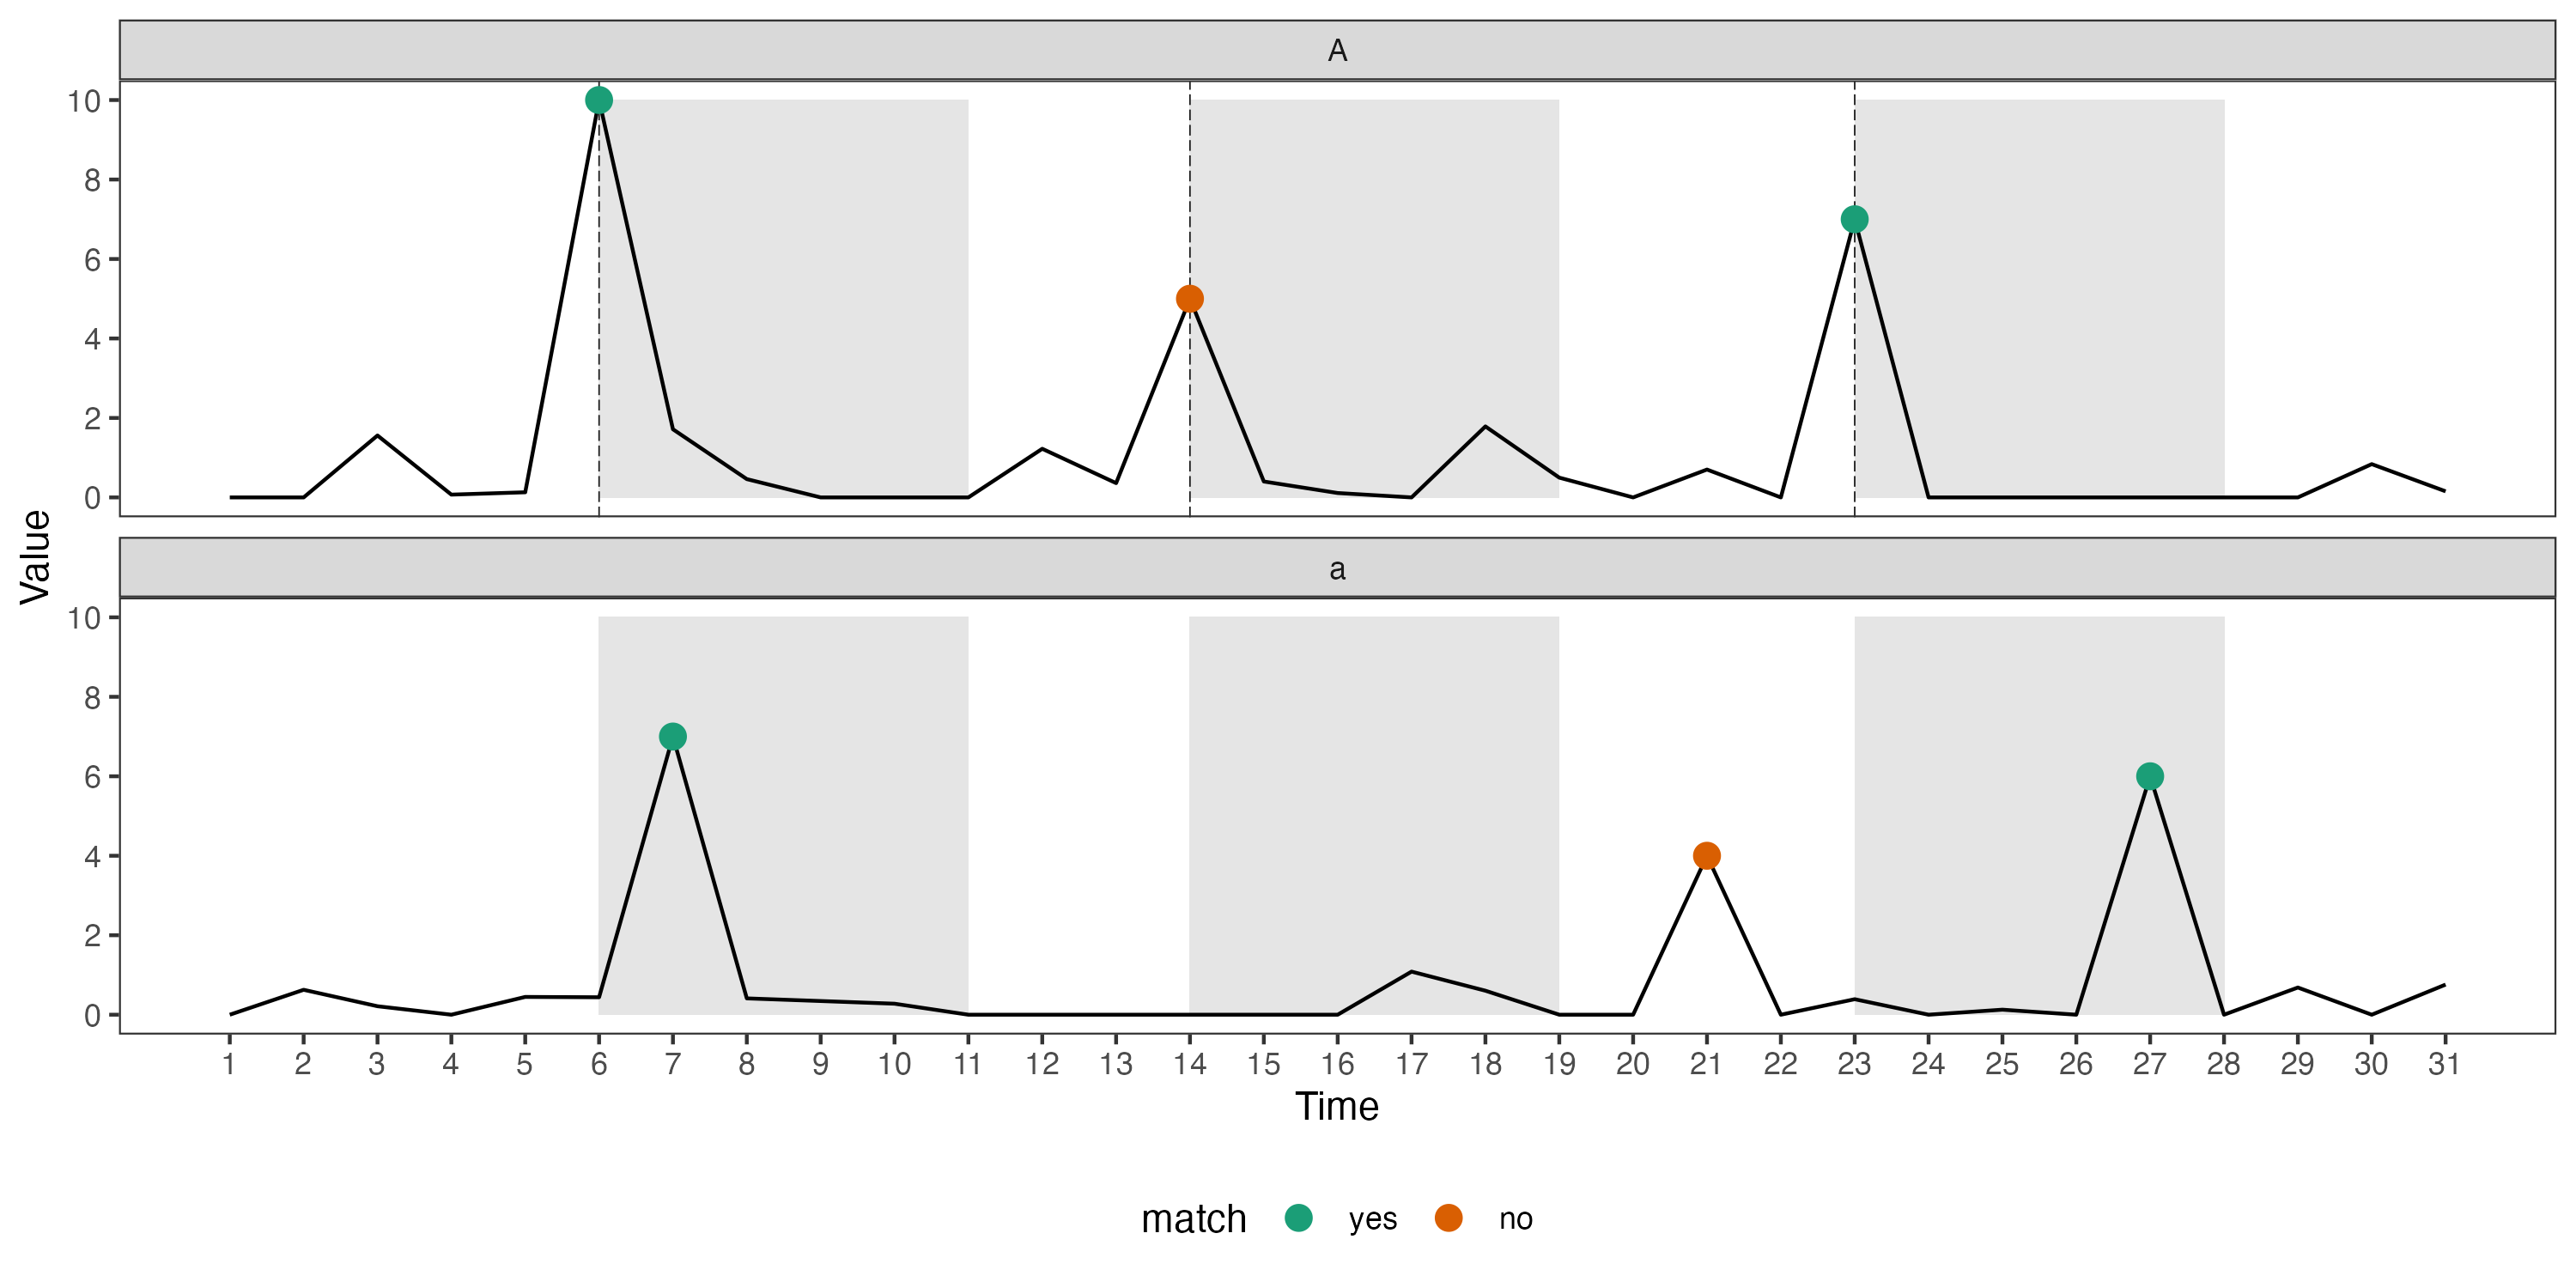
\includegraphics[width=1\linewidth]{figures/illu-matching} 

}

\caption{An illustration of temporal matching in cubble. Three highest peaks are identified in each series and intervals are constructed on series \code{A}. Two peaks in series \code{a} fall into the intervals and hence the two series are considered to have 2 matches.}\label{fig:illu-matching}
\end{figure}
\end{CodeChunk}

\begin{itemize}
\tightlist
\item
  \code{spatial_n_keep}: the number of spatial match for each site to
  keep
\item
  \code{spatial_dist_max}: the maximum distance allowed for a matched
  pair
\item
  \code{temporal_n_highest}: the number of peak used - 3 in the example
  above
\item
  \code{temporal_window}: the length of the interval - 5 in the example
  above
\item
  \code{temporal_min_match}: the minimum number of matched peak for a
  valid matched pair
\end{itemize}

This functionality can be seen as a matching exercise
\citep{stuart2010matching, mcintosh2018using} in the spatio-temporal
domain to pair up nearby observations. It can also be considered as a
form of data fusion \citep{cocchi2019data}, where data from multiple
sources are combined together.

\hypertarget{interactive-graphics}{%
\subsection{Interactive graphics}\label{interactive-graphics}}

Cubble fits in naturally with the interactive graphic pipeline discussed
in the literature
\citep{buja1988elements, buja1996interactive, sutherland2000orca, xie2014reactive, cheng2016enabling}.
Diagram \ref{fig:illu-interactive} illustrates how linking works from
the map to the time series in cubble. The map and time series plot is
associated with the nested or long cubble, respectively, and when a user
action is captured on the map, the site will be activated in the nested
cubble (left). The nested cubble will communicate to the long cubble to
activate all the observations with the same \code{id} (middle). The long
cubble will then highlight the activated series in the time series plot
(right).

The linking is also available from the time series plot to the map. The
selection(s) on the time series is through selecting the point(s) on the
time series and once a point is selected, it will be activated in the
long cubble. All the observations that share the same \code{id} are then
activated and this includes other points in the same time series in the
long cubble and the corresponding observation of site in the nested
cubble. These activated observations will then being reflected in the
updated plots and Diagram \ref{fig:illu-interactive-2} in the Appendix
illustrates this process.

\begin{CodeChunk}
\begin{figure}

{\centering 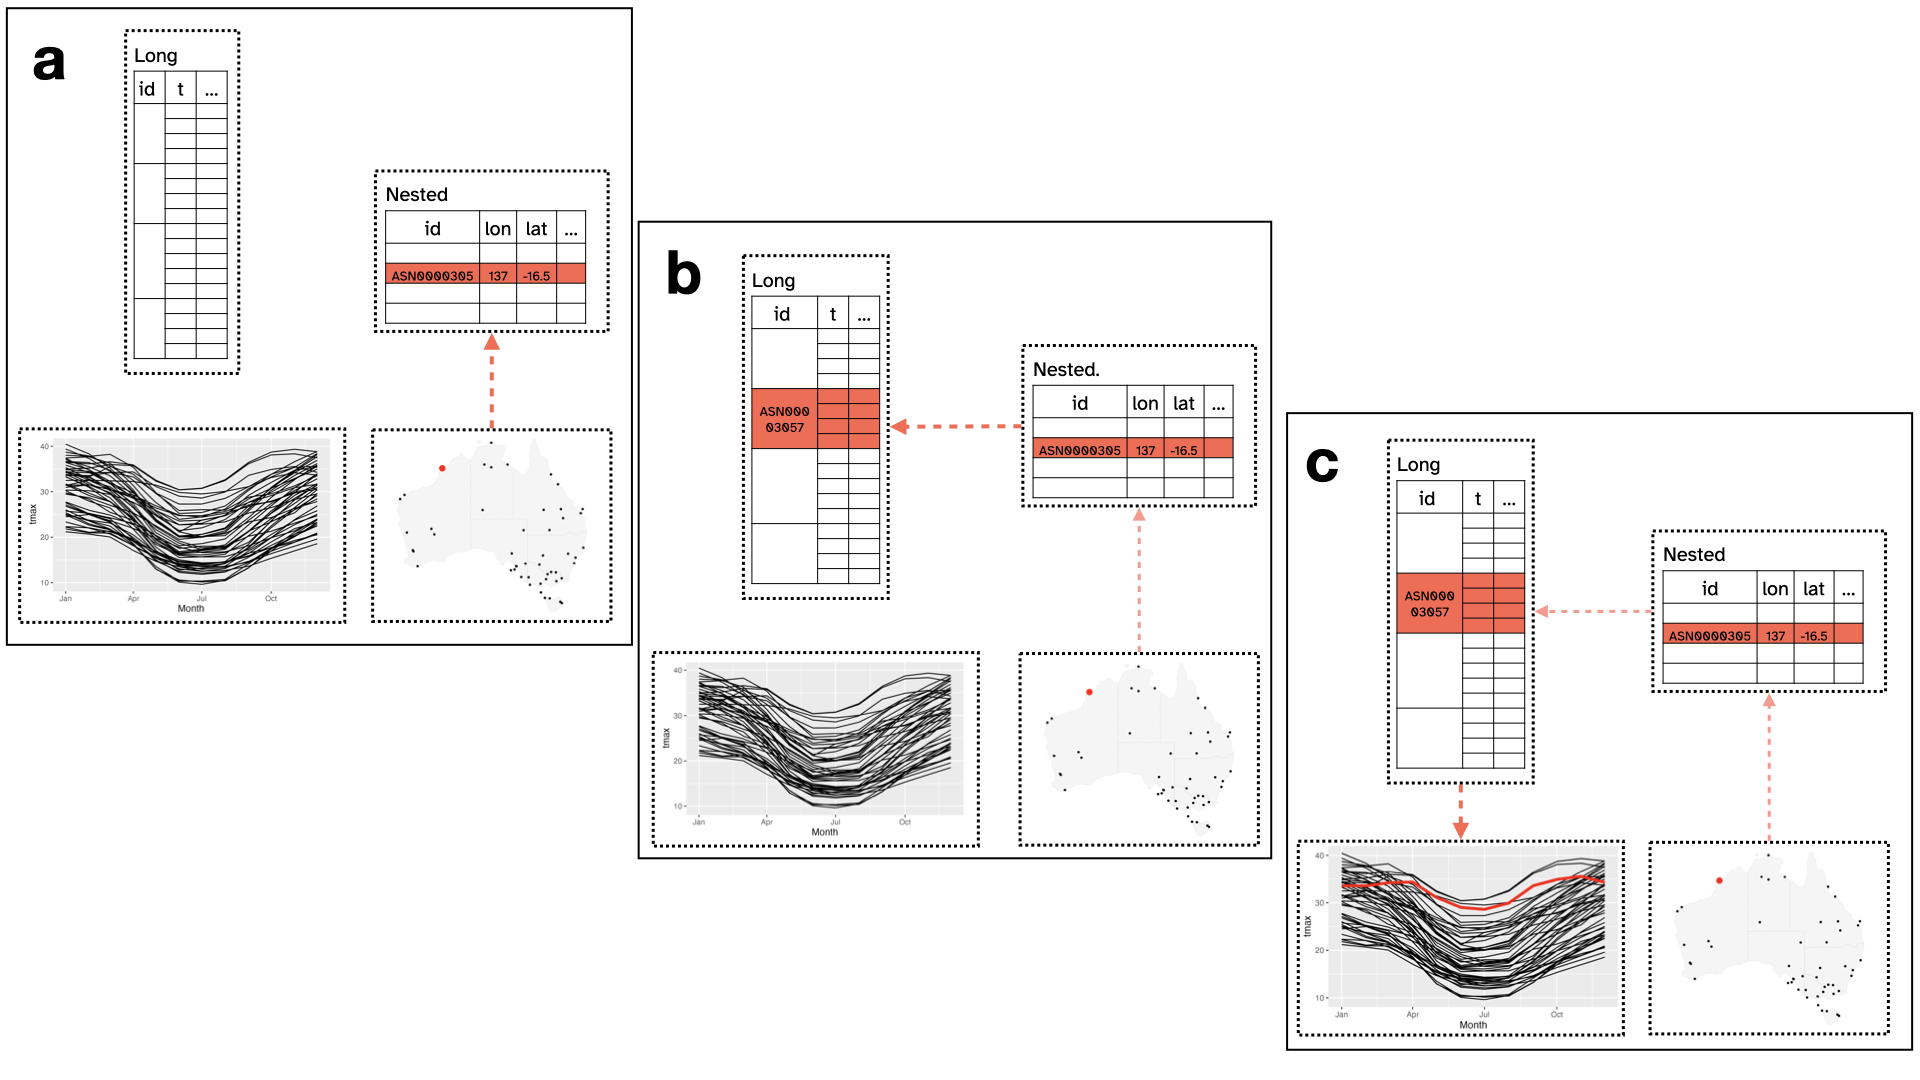
\includegraphics[width=1\linewidth,height=0.4\textheight]{/Users/sherryzhang/Documents/research/paper-cubble/figures/diagram-keynotes/diagram-keynotes.004} 

}

\caption[An illustration of the data model under interactive graphics with cubble]{An illustration of the data model under interactive graphics with cubble. The line plot and the map is made separately with the long and nested cubble. When a station is selected on the map (left), the corresponding row in the nested cubble will be activated. This will link to all the rows with the same id in the long cubble (middle) and update the line plot (right).}\label{fig:illu-interactive}
\end{figure}
\end{CodeChunk}

\hypertarget{st_transformation}{%
\subsection{Spatio-temporal transformations}\label{st_transformation}}

Spatio-temporal transformation is a useful technique to extract
information form spatio-temporal data. Glyph maps \citep{Wickham2012-yr}
transform the time coordinates into the space coordinates to plot the
time series of different locations on the map. Calendar plots
\citep{wang2020calendar} reconstructs time into calendar-based grid to
discover weekday and weekend pattern. Projection, or linear combination,
of variables summarises multivariate information into lower dimension to
further digest. This section elaborates on the glyph map.

In \proglang{R}, \pkg{GGally} implements glyph maps through the
\code{glyphs()} function. The function constructs a data frame with
calculated position (\code{gx}. \code{gy}. \code{gid}) of each point on
the time series using linear algebra (Equation 1 and 2 in
\citet{Wickham2012-yr}). The data can then be piped into \code{ggplot}
to create the glyph map as:

\begin{CodeChunk}
\begin{CodeInput}
R> library(ggplot2)
R> gly <- glyphs(data, 
+               x_major = ..., x_minor = ..., 
+               y_major = ..., y_minor = ..., ...)
R> 
R> ggplot(gly, aes(gx, gy, group = gid)) + 
+   geom_path() 
\end{CodeInput}
\end{CodeChunk}

A re-implementation of the glyph map as a ggproto, \code{GeomGlyph}, has
been made in the \pkg{cubble} package and now the glyph map can be
created with \code{geom_glyph()}:

\begin{CodeChunk}
\begin{CodeInput}
R> ggplot(data = data) +
+   geom_glyph(aes(x_major = ..., x_minor = ..., 
+                  y_major = ..., y_minor = ...))
\end{CodeInput}
\end{CodeChunk}

Some useful controls over the glyph map is also available in the
\code{geom_glyph()} implementation. Polar glyph map can be specify as a
parameter, \code{polar = TRUE}. in the \code{geom_glyph()}, along with
\code{width} and \code{height} in either absolute or relative value.
Global and local scale can be controlled by the parameter
\code{global_rescale}. which default to \code{TRUE} for global scaling.
Reference box and line can be added with separate
\code{geom_glyph_box()} and \code{geom_glyph_line()}.

\hypertarget{examples}{%
\section{Examples}\label{examples}}

\hypertarget{australia-historical-maximum-temperature}{%
\subsection{Australia historical maximum
temperature}\label{australia-historical-maximum-temperature}}

Global Historical Climatology Network (GHCN) provides daily climate
measures from stations across the world. The dataset
\code{weatherdata::historical_tmax} extracts the maximum temperature for
236 Australian stations from GHCN with starting from year 1969.
\code{weatherdata::historical_tmax} is already in a cubble, with
\code{id} as the key, \code{date} as the index, and
\code{c(longitude, latitude)} as the coordinates. This example compares
the maximum temperature in two periods: 1971 - 1975 and 2016 - 2020 for
stations in Victoria and New South Wales.

Stations in the two states can be subsetted by the station number:
Australia GHCN station number starts with ``ASN00'' and followed by the
\href{http://www.bom.gov.au/climate/cdo/about/site-num.shtml}{Bureau of
Meteorology (BOM) station number}, where the 2nd and 3rd digit (7th and
8th in the GHCN number) define the state of the station. New South Wales
stations start from 46 to 75 and Victoria stations follow from 76 to 90.
Filtering Victoria and New South Wales stations is an operation in the
spatial dimension and hence uses the nested form:

\begin{CodeChunk}
\begin{CodeInput}
R> tmax <- weatherdata::historical_tmax %>%
+   filter(between(stringr::str_sub(id, 7, 8), 46, 90))
\end{CodeInput}
\end{CodeChunk}

Filtering for the period 1971 \textasciitilde{} 1975 and 2016
\textasciitilde{} 2020 is an operation on the time dimension and the
nested cubble needs to be switched to the long cubble by
\code{stretch()}:

\begin{CodeChunk}
\begin{CodeInput}
R> tmax <- tmax %>% 
+   stretch() %>%
+   filter(lubridate::year(date) %in% c(1971:1975, 2016:2020)) 
\end{CodeInput}
\end{CodeChunk}

A monthly average is used for both periods to smooth the maximum
temperature and it is again an operation on the time dimension:

\begin{CodeChunk}
\begin{CodeInput}
R> tmax <- tmax %>%
+   group_by(month = lubridate::month(date), 
+          group = as.factor(ifelse(lubridate::year(date) > 2015, 
+                                   "2016 ~ 2020", "1971 ~ 1975"))) %>%
+   summarise(tmax = mean(tmax, na.rm = TRUE))
\end{CodeInput}
\end{CodeChunk}

A few stations don't have records during 1971 - 1975 and further
investigation shows that while the first and last year of each series is
recorded, the missing years in this period is not reported. These
stations are filtered out by examining whether the summarised time
series has a total of 24 months. The long cubble needs to be switched to
the nested form for this spatial operation using \code{tamp()}:

\begin{CodeChunk}
\begin{CodeInput}
R> tmax <- tmax %>% tamp() %>% filter(nrow(ts) == 24) 
\end{CodeInput}
\end{CodeChunk}

Lastly, to create a glyph map, both the major (\code{longitude},
\code{latitude}) and minor (\code{month}, \code{tmax}) coordinates need
to be in the same table. Spatial variables can be moved to the long form
with \code{migrate()}:

\begin{CodeChunk}
\begin{CodeInput}
R> tmax <- tmax %>% stretch() %>% migrate(latitude, longitude)
\end{CodeInput}
\end{CodeChunk}

\code{tmax} can then be supplied to \code{geom_glyph()} for the glyph
map in Figure \ref{fig:basic-manip} with a station inset on the top left
corner:

\begin{CodeChunk}
\begin{CodeInput}
R> nsw_vic <- ozmaps::abs_ste %>% 
+   filter(NAME %in% c("Victoria", "New South Wales"))
R> 
R> ggplot() + 
+   geom_sf(data = nsw_vic, 
+           fill = "transparent", color = "grey", linetype = "dotted") + 
+   geom_glyph(data = tmax, 
+              aes(x_major = longitude, x_minor = month, 
+                  y_major = latitude, y_minor = tmax,
+                  group = interaction(id, group), color = group),
+              width = 1, height = 0.5) +
+   ...
\end{CodeInput}
\end{CodeChunk}

\begin{CodeChunk}
\begin{figure}

{\centering 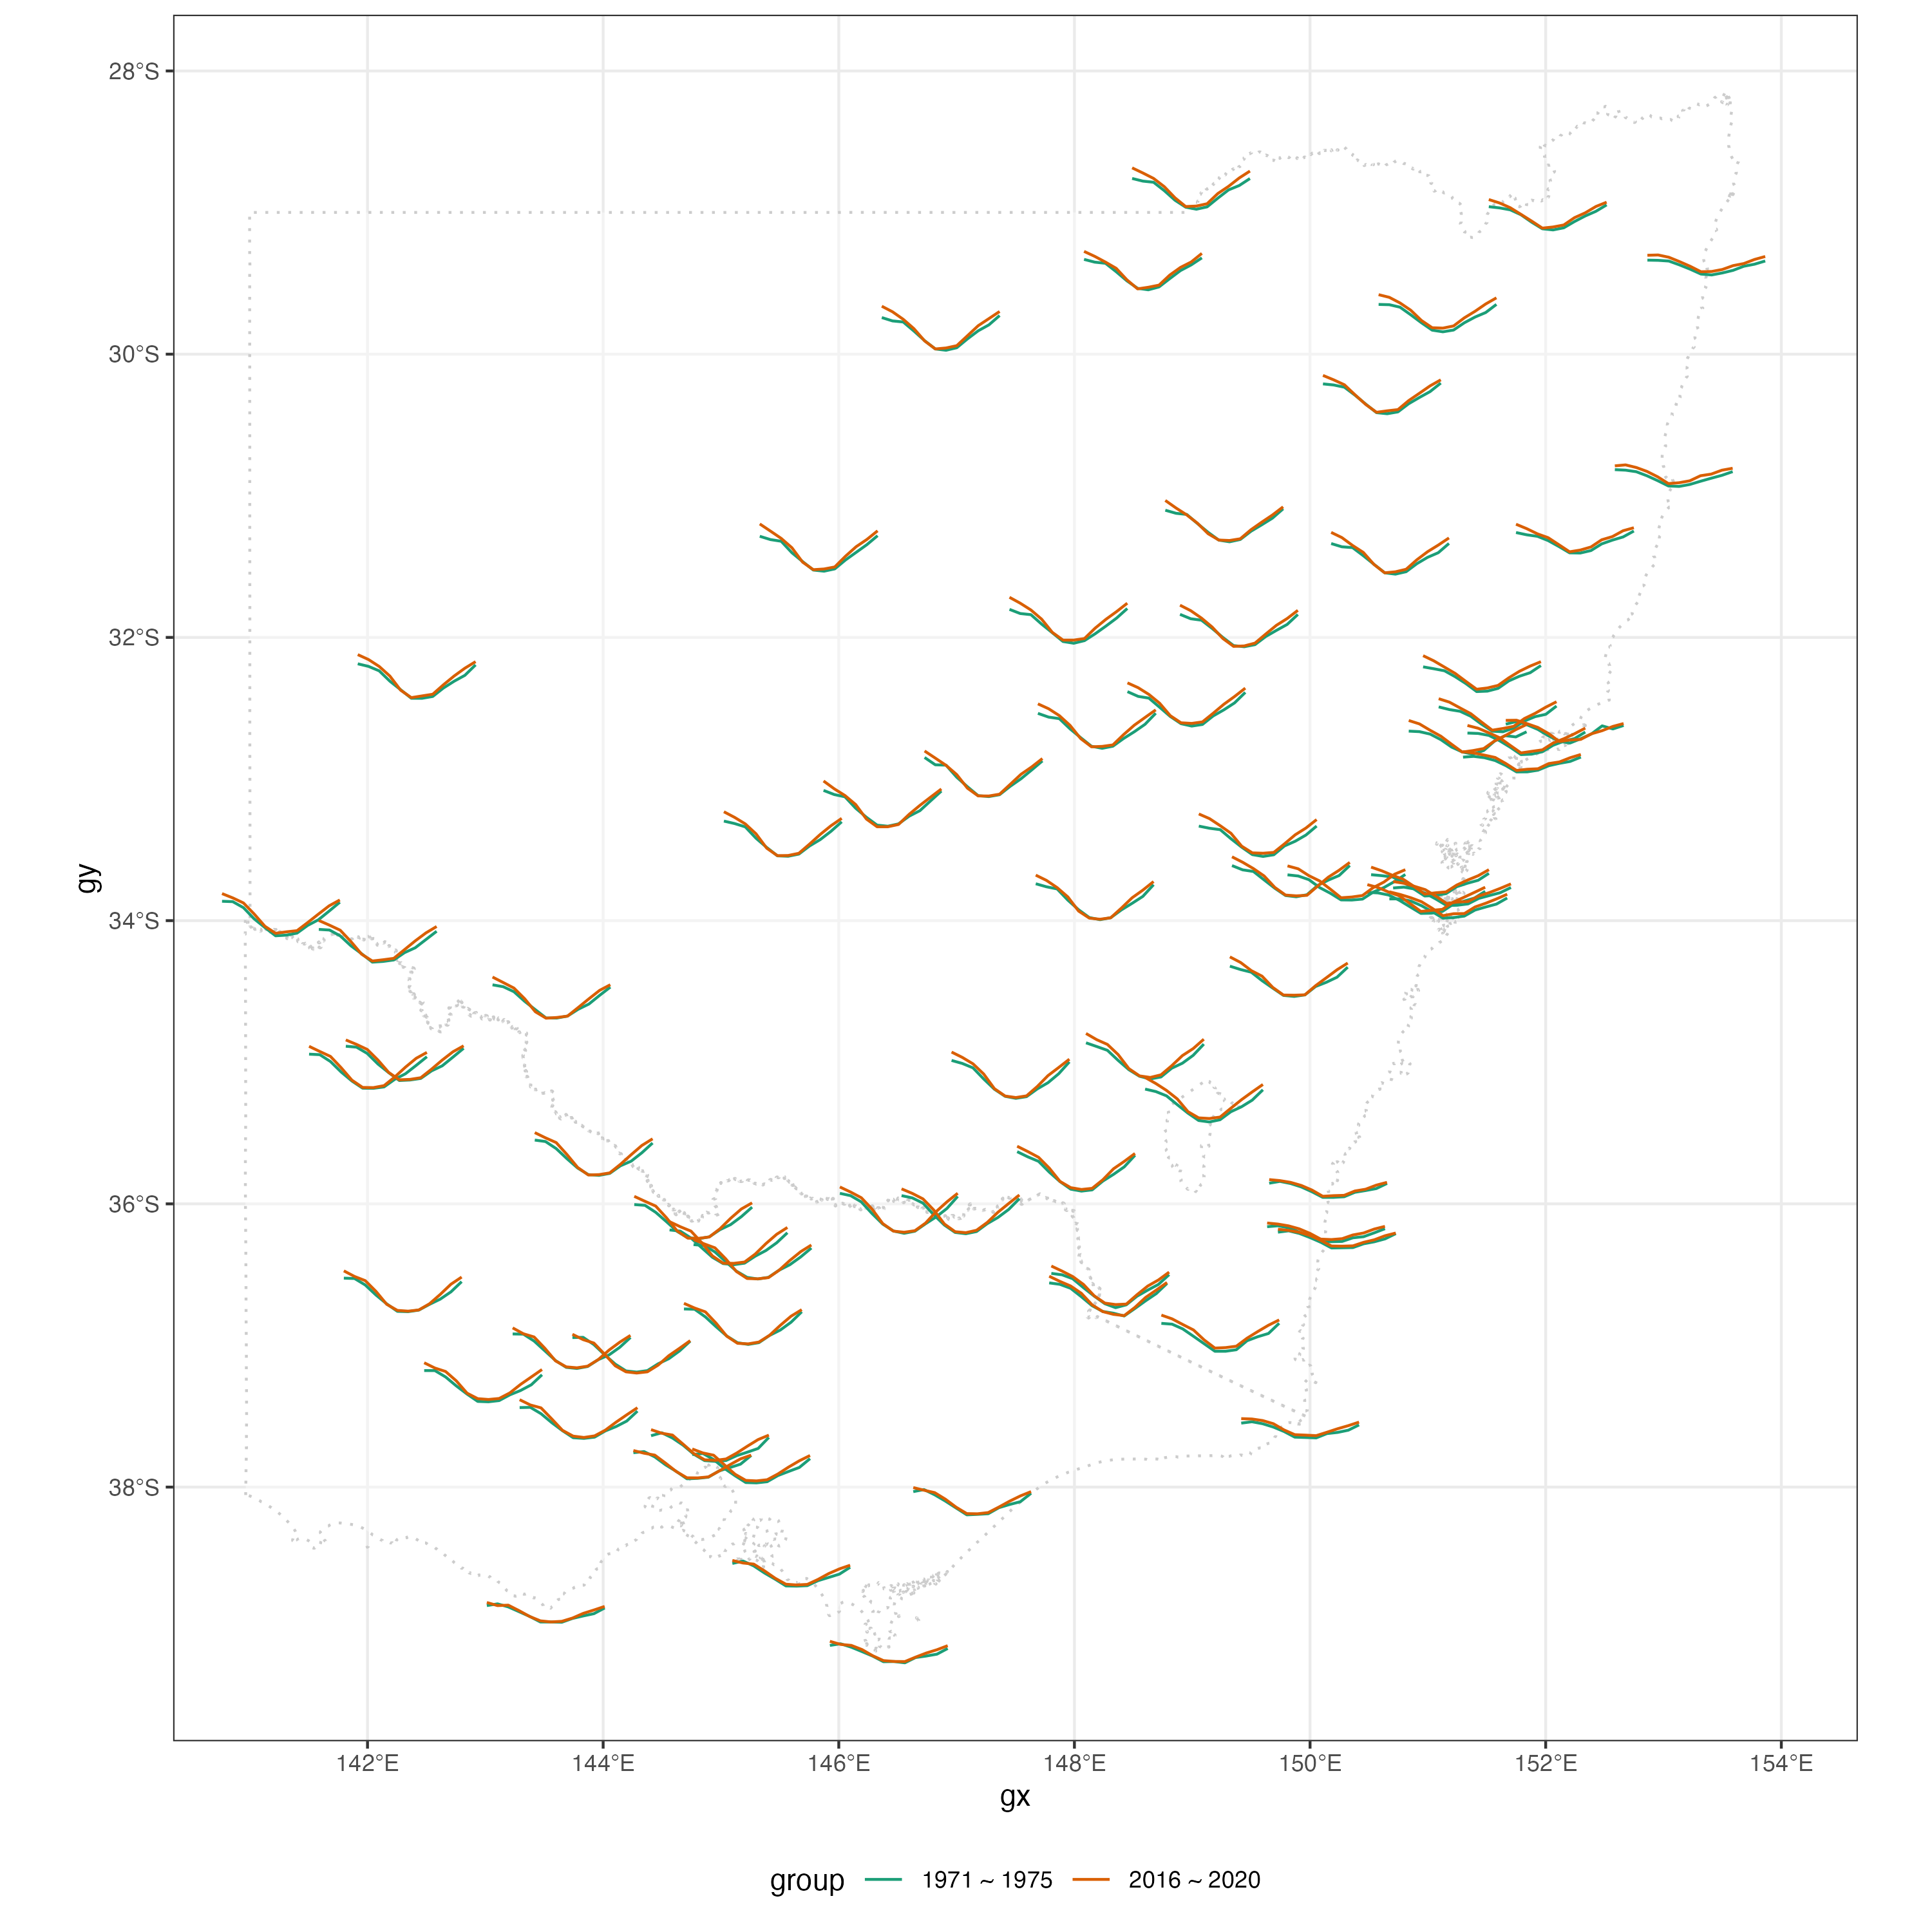
\includegraphics[width=1\linewidth,height=0.7\textheight]{figures/basic-manip} 

}

\caption[A glyph map of the average maximum temperature by month of Victoria and New South Wales weather stations in Australia]{A glyph map of the average maximum temperature by month of Victoria and New South Wales weather stations in Australia. On the top left corner is an insetted plot of station Cobar highlighted in the black box.}\label{fig:basic-manip}
\end{figure}
\end{CodeChunk}

\hypertarget{australia-precipitation-pattern-in-2020}{%
\subsection{Australia precipitation pattern in
2020}\label{australia-precipitation-pattern-in-2020}}

In the previous example, there has already been some overlapping of the
glyphs for a few stations near (151E, 34S) and (152E, 33S) and this will
be a problem when mapping more stations in the national level.
Aggregation can be helpful to group series into clusters before
visualising the cluster with glyph map. This example shows how to
organise data at both level with \code{switch_key()}.

\code{weatherdata::climate_full}, also extracted from GHCN, records
daily precipitation and maximum/ minimum temperature for 639 stations in
Australia from 2016 to 2020. A simple kmean algorithm based on the
distance matrix is used to create 20 clusters. This creates
\code{station_nested} as a station level nested cubble with a cluster
column indicating the group each station belongs to. More complex
algorithms can be used for other problem, as long as there is a mapping
from each station to a cluster.

\begin{CodeChunk}
\begin{CodeInput}
R> station_nested <- weatherdata::climate_full %>% 
+   mutate(cluster = ...)
\end{CodeInput}
\end{CodeChunk}

To create a group level cubble, use \code{switch_key()} with the new key
variable, \code{cluster}:

\begin{CodeChunk}
\begin{CodeInput}
R> cluster_nested <- station_nested %>% switch_key(cluster) 
\end{CodeInput}
\end{CodeChunk}

With the group level cubble, \code{get_centroid()} is useful to compute
the centroid of each cluster, which will be used as the major axis for
the glyph map later:

\begin{CodeChunk}
\begin{CodeInput}
R> cluster_nested <- cluster_nested %>% get_centroid()
\end{CodeInput}
\end{CodeChunk}

Long form cubble at both levels can be accessed through stretching the
nested form and with access to both station and cluster level cubbles,
various plots can be made to understand the cluster. Figure
\ref{fig:basic-agg} shows two example plots that can be made with this
data: subplot A is a glyph map made with the cluster level cubble in the
long form and subplot B inspects the station membership of each cluster
using the station level cubble in the nested form.

\begin{CodeChunk}
\begin{figure}

{\centering 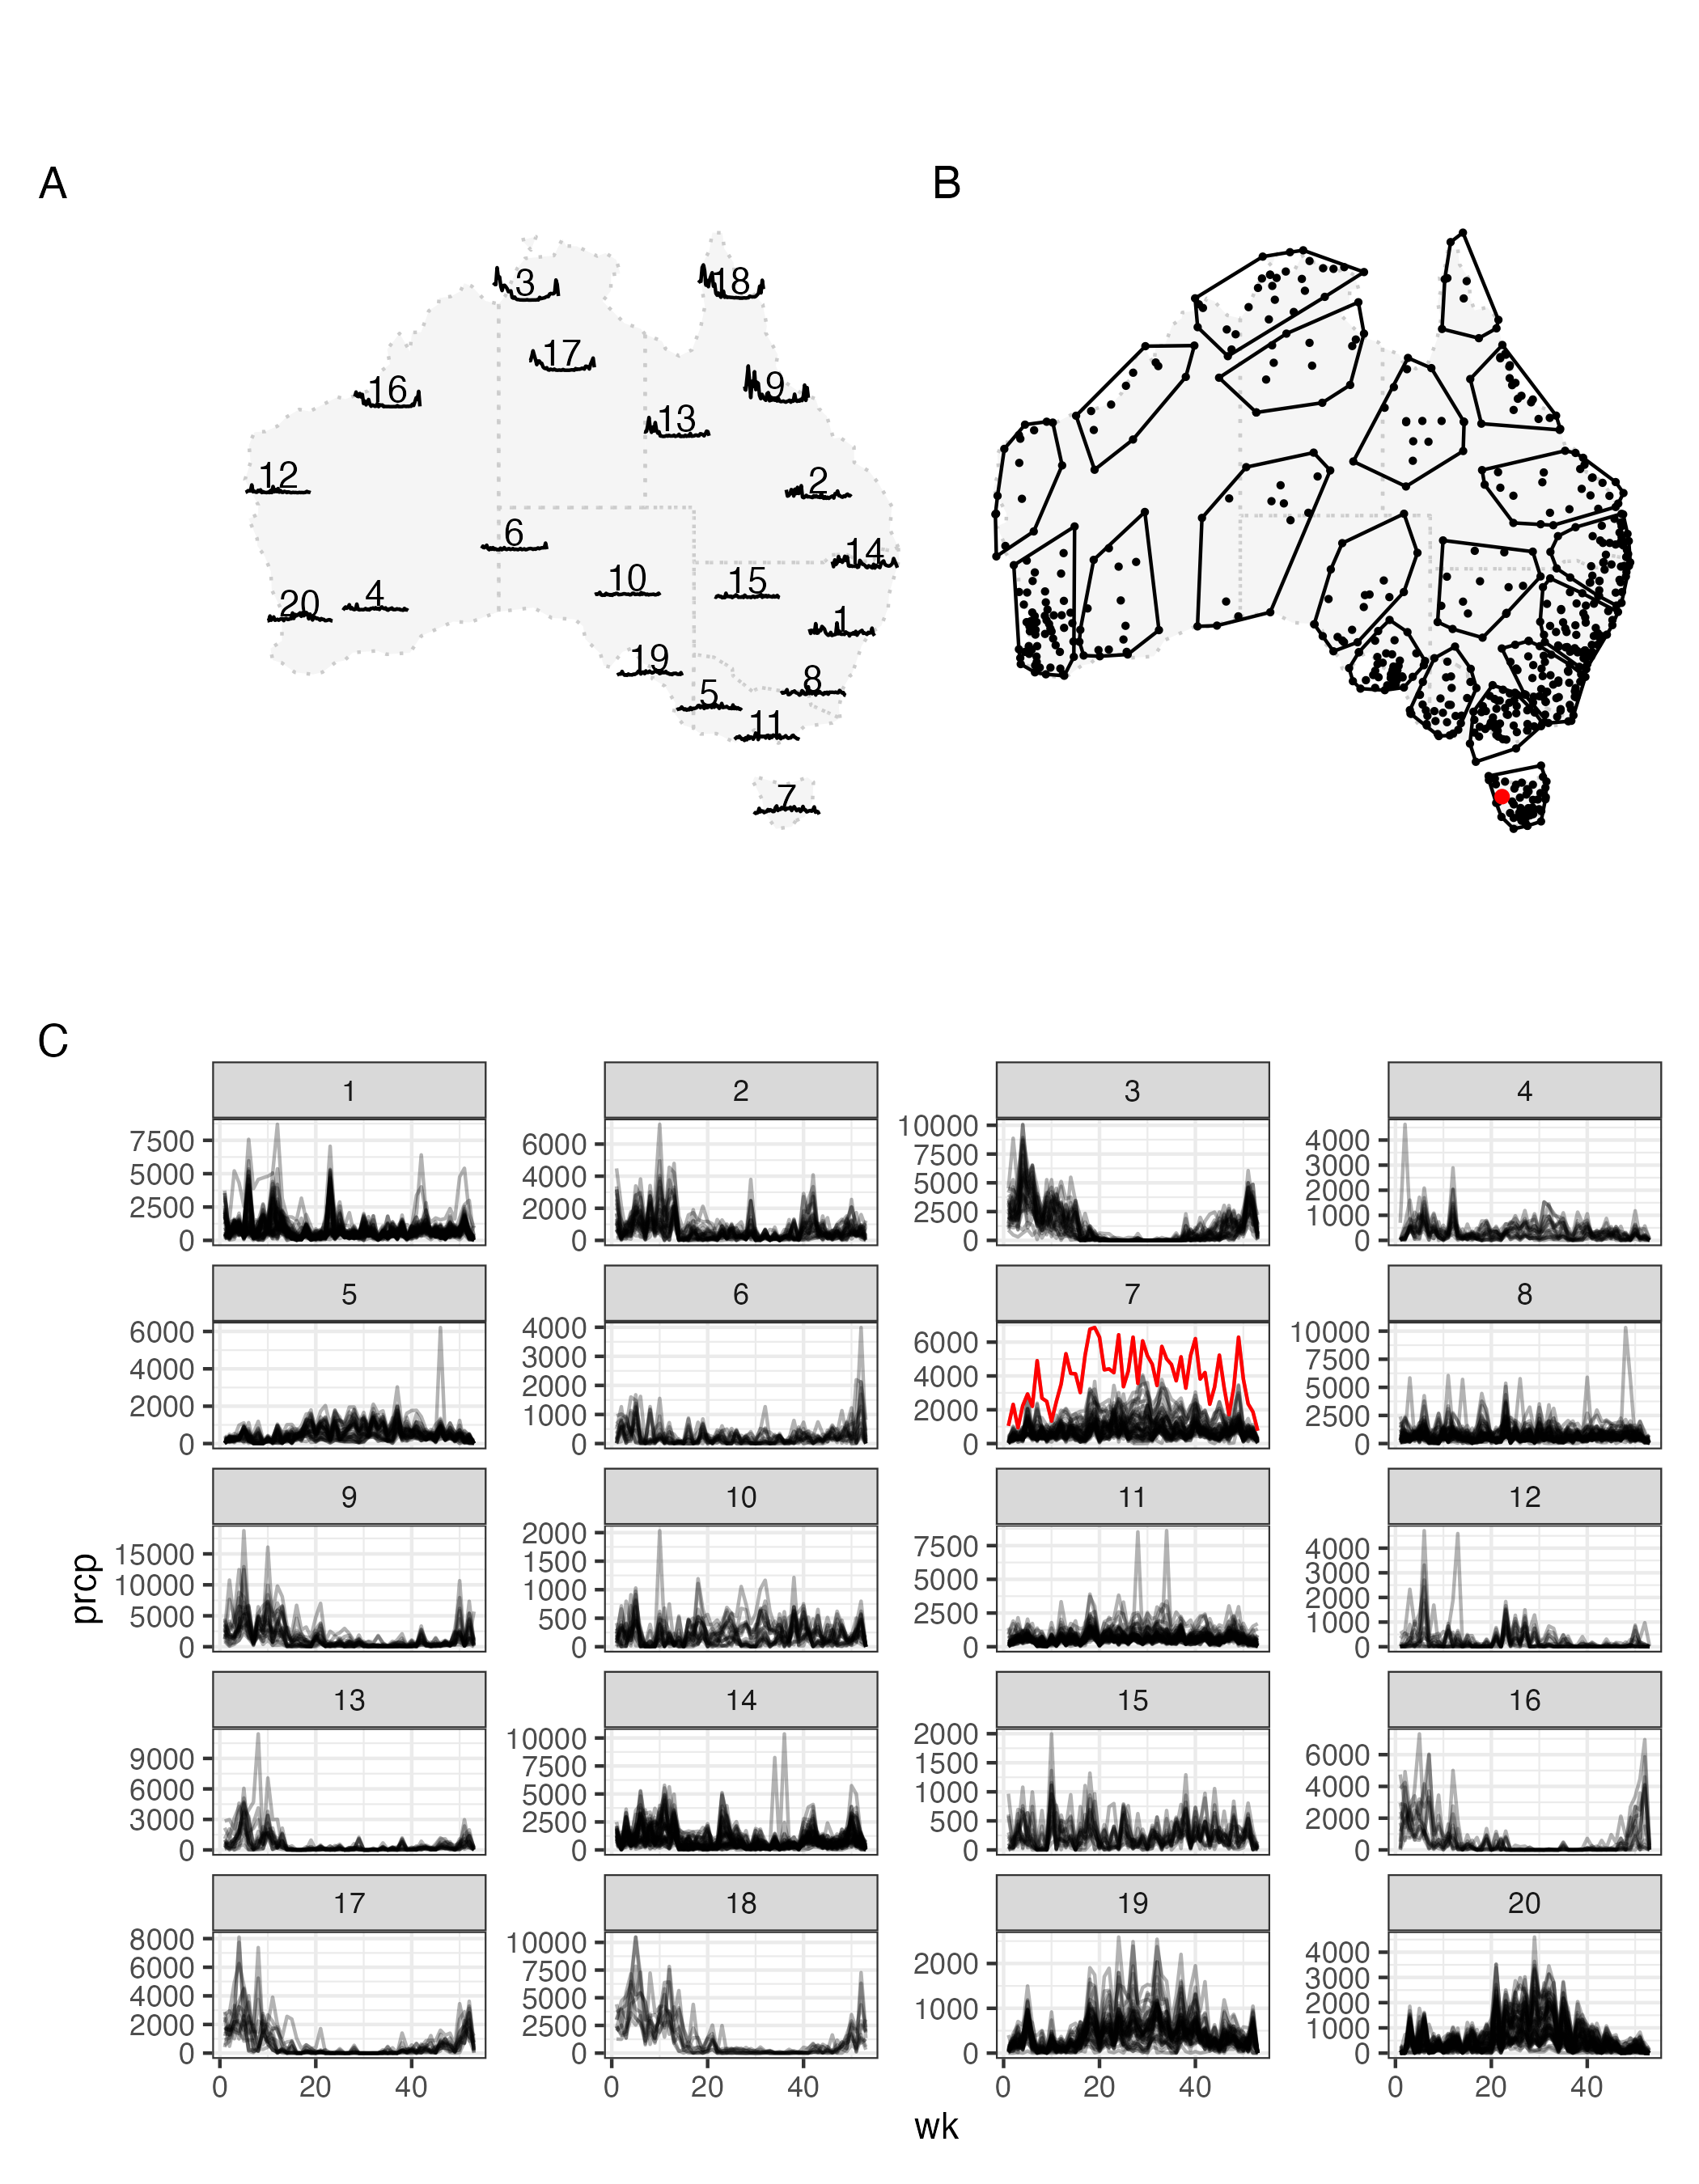
\includegraphics[width=1\linewidth]{figures/basic-agg} 

}

\caption[Profile of aggregated precipitation from 639 weather stations in Australia]{Profile of aggregated precipitation from 639 weather stations in Australia. Subplot A shows the glyph map of the weekly averaged precipitation of each cluster. The group number of printed in the middle of y minor axis and can be used as a reference line to read the magnitude. Subplot B shows the station membership of each cluster.}\label{fig:basic-agg}
\end{figure}
\end{CodeChunk}

\hypertarget{river-level-data-in-victoria-water-gauges}{%
\subsection{River level data in Victoria water
gauges}\label{river-level-data-in-victoria-water-gauges}}

Bureau of Meteorology collects
\href{http://www.bom.gov.au/metadata/catalogue/19115/ANZCW0503900528?template=full}{water
data} from river gauges and this includes variables: electrical
conductivity, turbidity, water course discharge, water course level, and
water temperature. In particular, water level will interactive with
precipitation from the climate data since rainfall will raise the water
level in the river. Figure \ref{fig:matching-map} gives the location of
available weather station and water gauges in Victoria.

\begin{CodeChunk}
\begin{figure}

{\centering 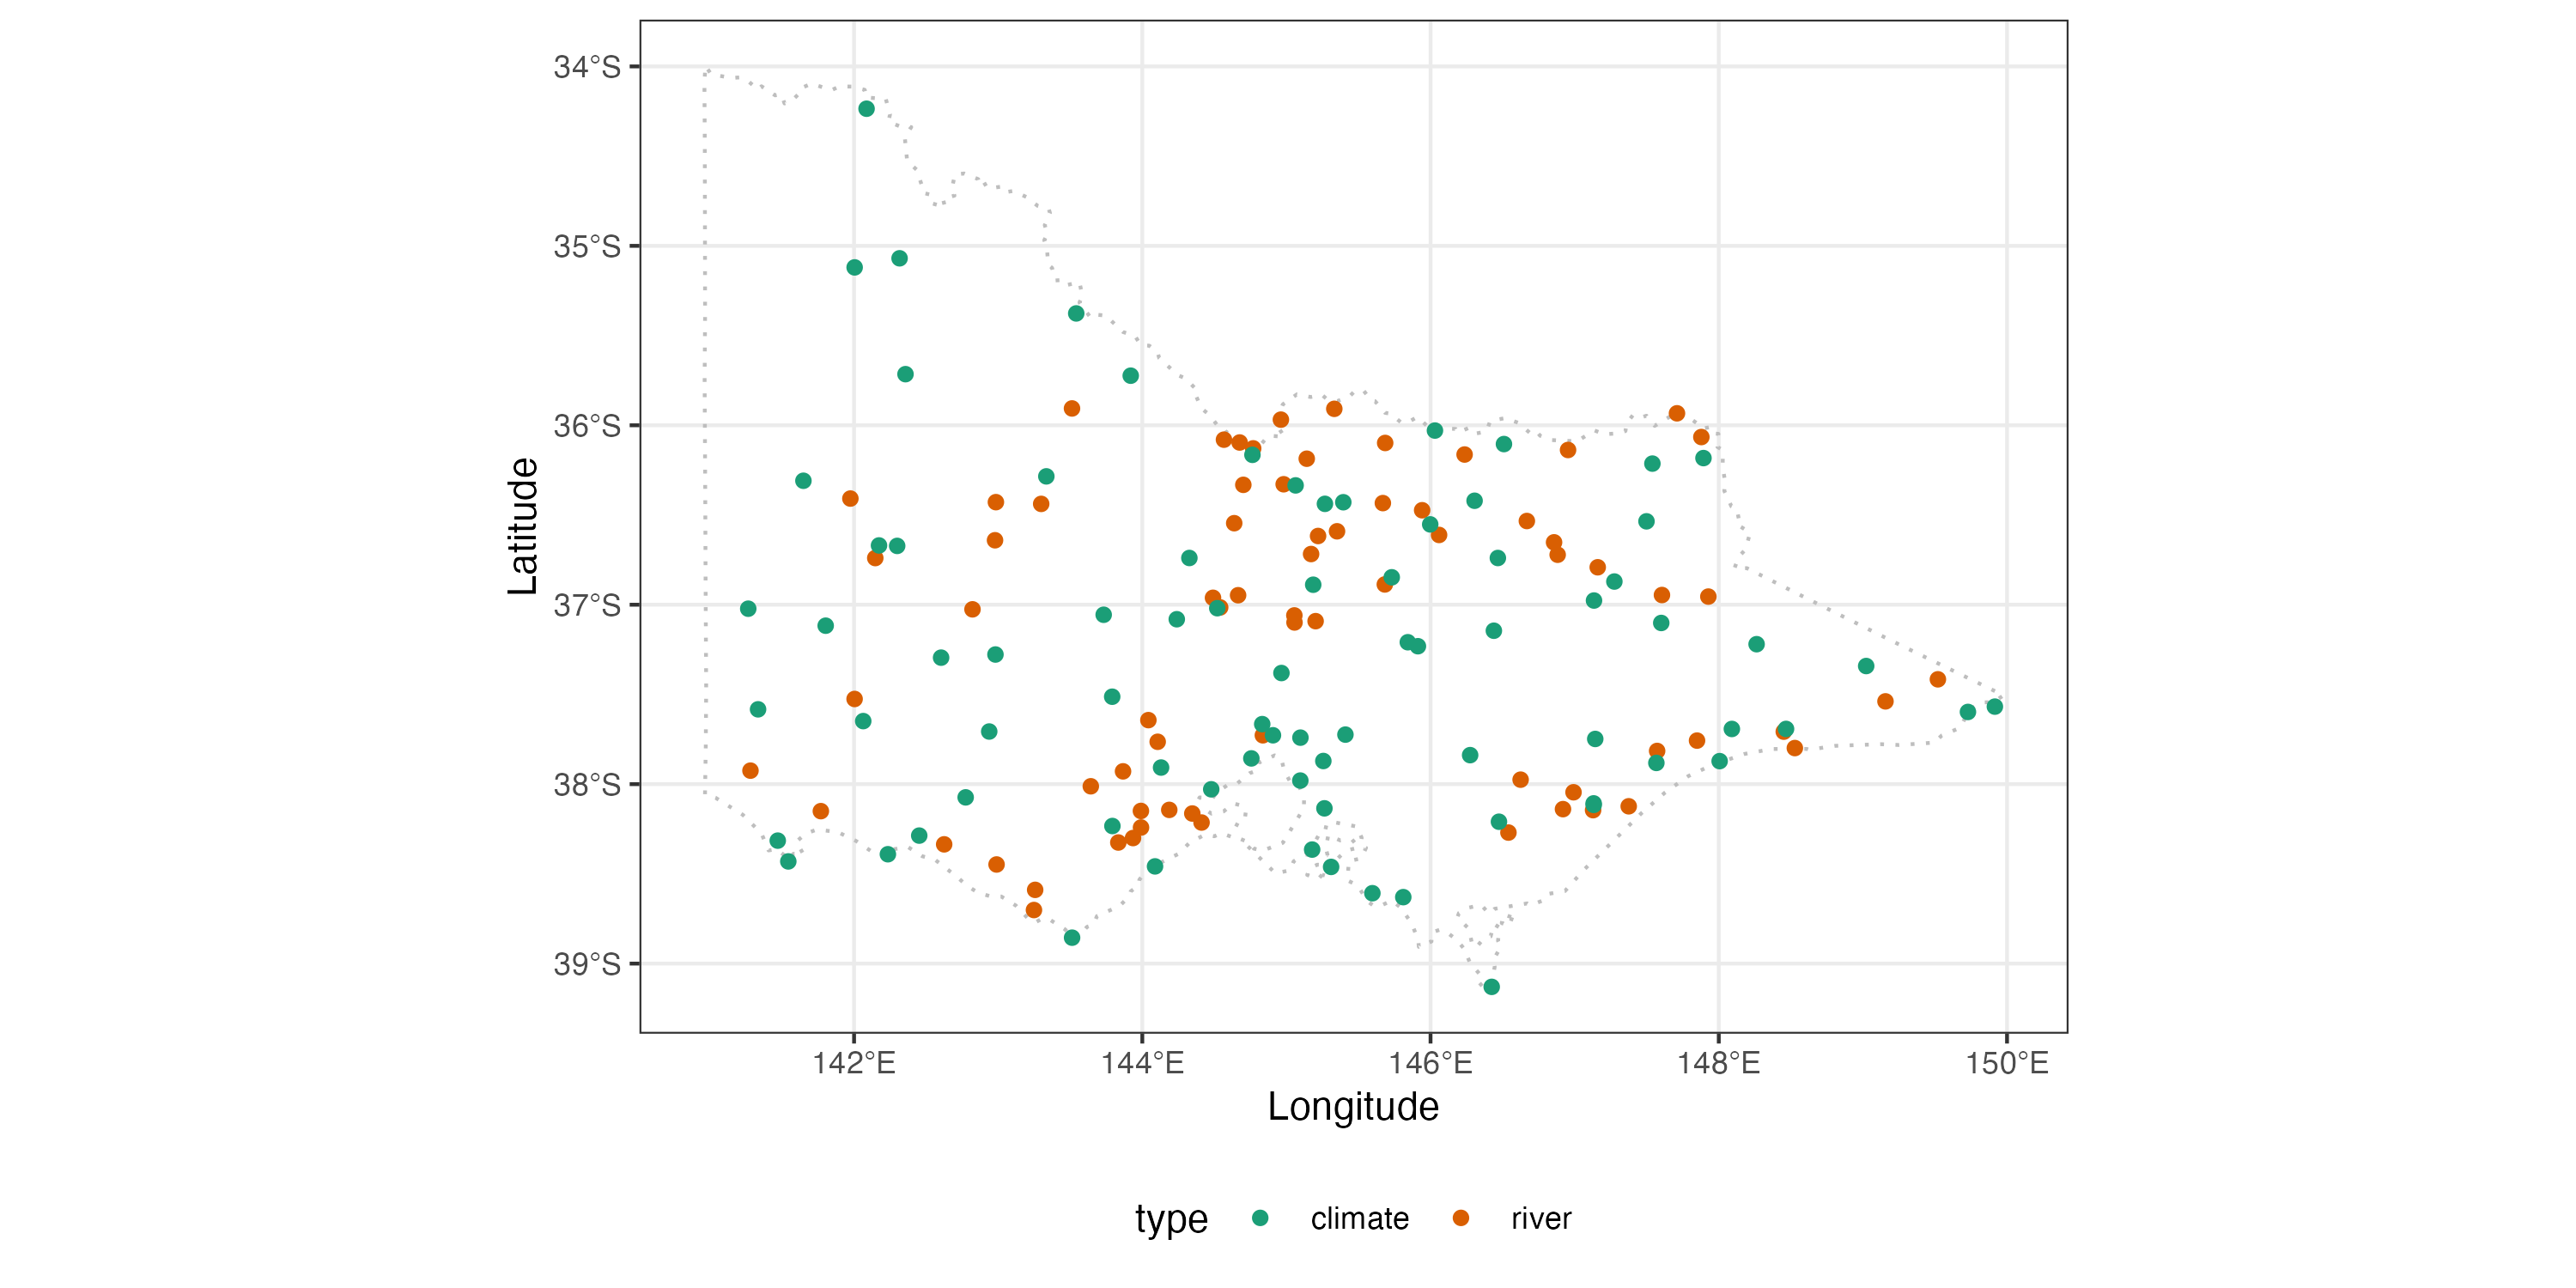
\includegraphics[width=1\linewidth]{figures/matching-map} 

}

\caption[Location of weather stations and river gauges in Victoria, Australia]{Location of weather stations and river gauges in Victoria, Australia.}\label{fig:matching-map}
\end{figure}
\end{CodeChunk}

From the map, a few water gauges and weather stations are close to each
other and the fluctuation of the water level could be matched up with
precipitation measured by the climate station. As introduced in Section
3.2, \code{match_sites()} can be used to match one source of data with
another source in a cubble. Here \code{Water_course_level} in
\code{river} will be matched to \code{prcp} in \code{climate} in 2020.
The two datasets need to be specified as the first two arguments and the
variable to match can be specified in \code{temporal_by} using the
\code{by} syntax in \code{join}. \code{temporal_independent} controls
the variable used to construct the interval and the goal here is to see
if precipitation will be reflected by the water level in the river. This
puts precipitation \code{prcp}, as the independent. Given there is one
year worth of data, the number of peak (\code{temporal_n_highest}) to
consider is slightly raised from a default 20 to 30 and
\code{temporal_min_match} is raised accordingly To return all the pairs
of the match, \code{temporal_min_match} can be set to 0.

\begin{CodeChunk}
\begin{CodeInput}
R> res <- match_sites(
+   river, climate,
+   temporal_by = c("Water_course_level" = "prcp"),
+   temporal_independent = "prcp",  
+   temporal_n_highest = 30,
+   temporal_min_match = 15
+ )
\end{CodeInput}
\end{CodeChunk}

The output from matching is also a cubble, with additional column
\code{dist} and \code{group} produced from spatial matching and
\code{n_match} from temporal matching.

\begin{CodeChunk}
\begin{CodeOutput}
# cubble:   id [8]: nested form
# bbox:     [144.52, -37.73, 146.06, -36.55]
# temporal: date [date], matched_var [dbl]
  id          name                lat  long type    dist group ts        n_match
  <chr>       <chr>             <dbl> <dbl> <chr>  <dbl> <int> <list>      <int>
1 405234      SEVEN CREEKS @ D~ -36.9  146. river   6.15     5 <tibble ~      21
2 404207      HOLLAND CREEK @ ~ -36.6  146. river   8.54    10 <tibble ~      21
3 ASN00082042 strathbogie       -36.8  146. clima~  6.15     5 <tibble ~      21
4 ASN00082170 benalla airport   -36.6  146. clima~  8.54    10 <tibble ~      21
5 230200      MARIBYRNONG RIVE~ -37.7  145. river   6.17     6 <tibble ~      19
6 ASN00086038 essendon airport  -37.7  145. clima~  6.17     6 <tibble ~      19
7 406213      CAMPASPE RIVER @~ -37.0  145. river   1.84     1 <tibble ~      18
8 ASN00088051 redesdale         -37.0  145. clima~  1.84     1 <tibble ~      18
\end{CodeOutput}
\end{CodeChunk}

Figure \ref{fig:matching} plots the matched pairs on the map or to view
the matched series. There are four pairs of matches, which all locates
in the middle Victoria and the concurrent increase of precipitation and
water level can be observed.

\begin{CodeChunk}
\begin{figure}

{\centering 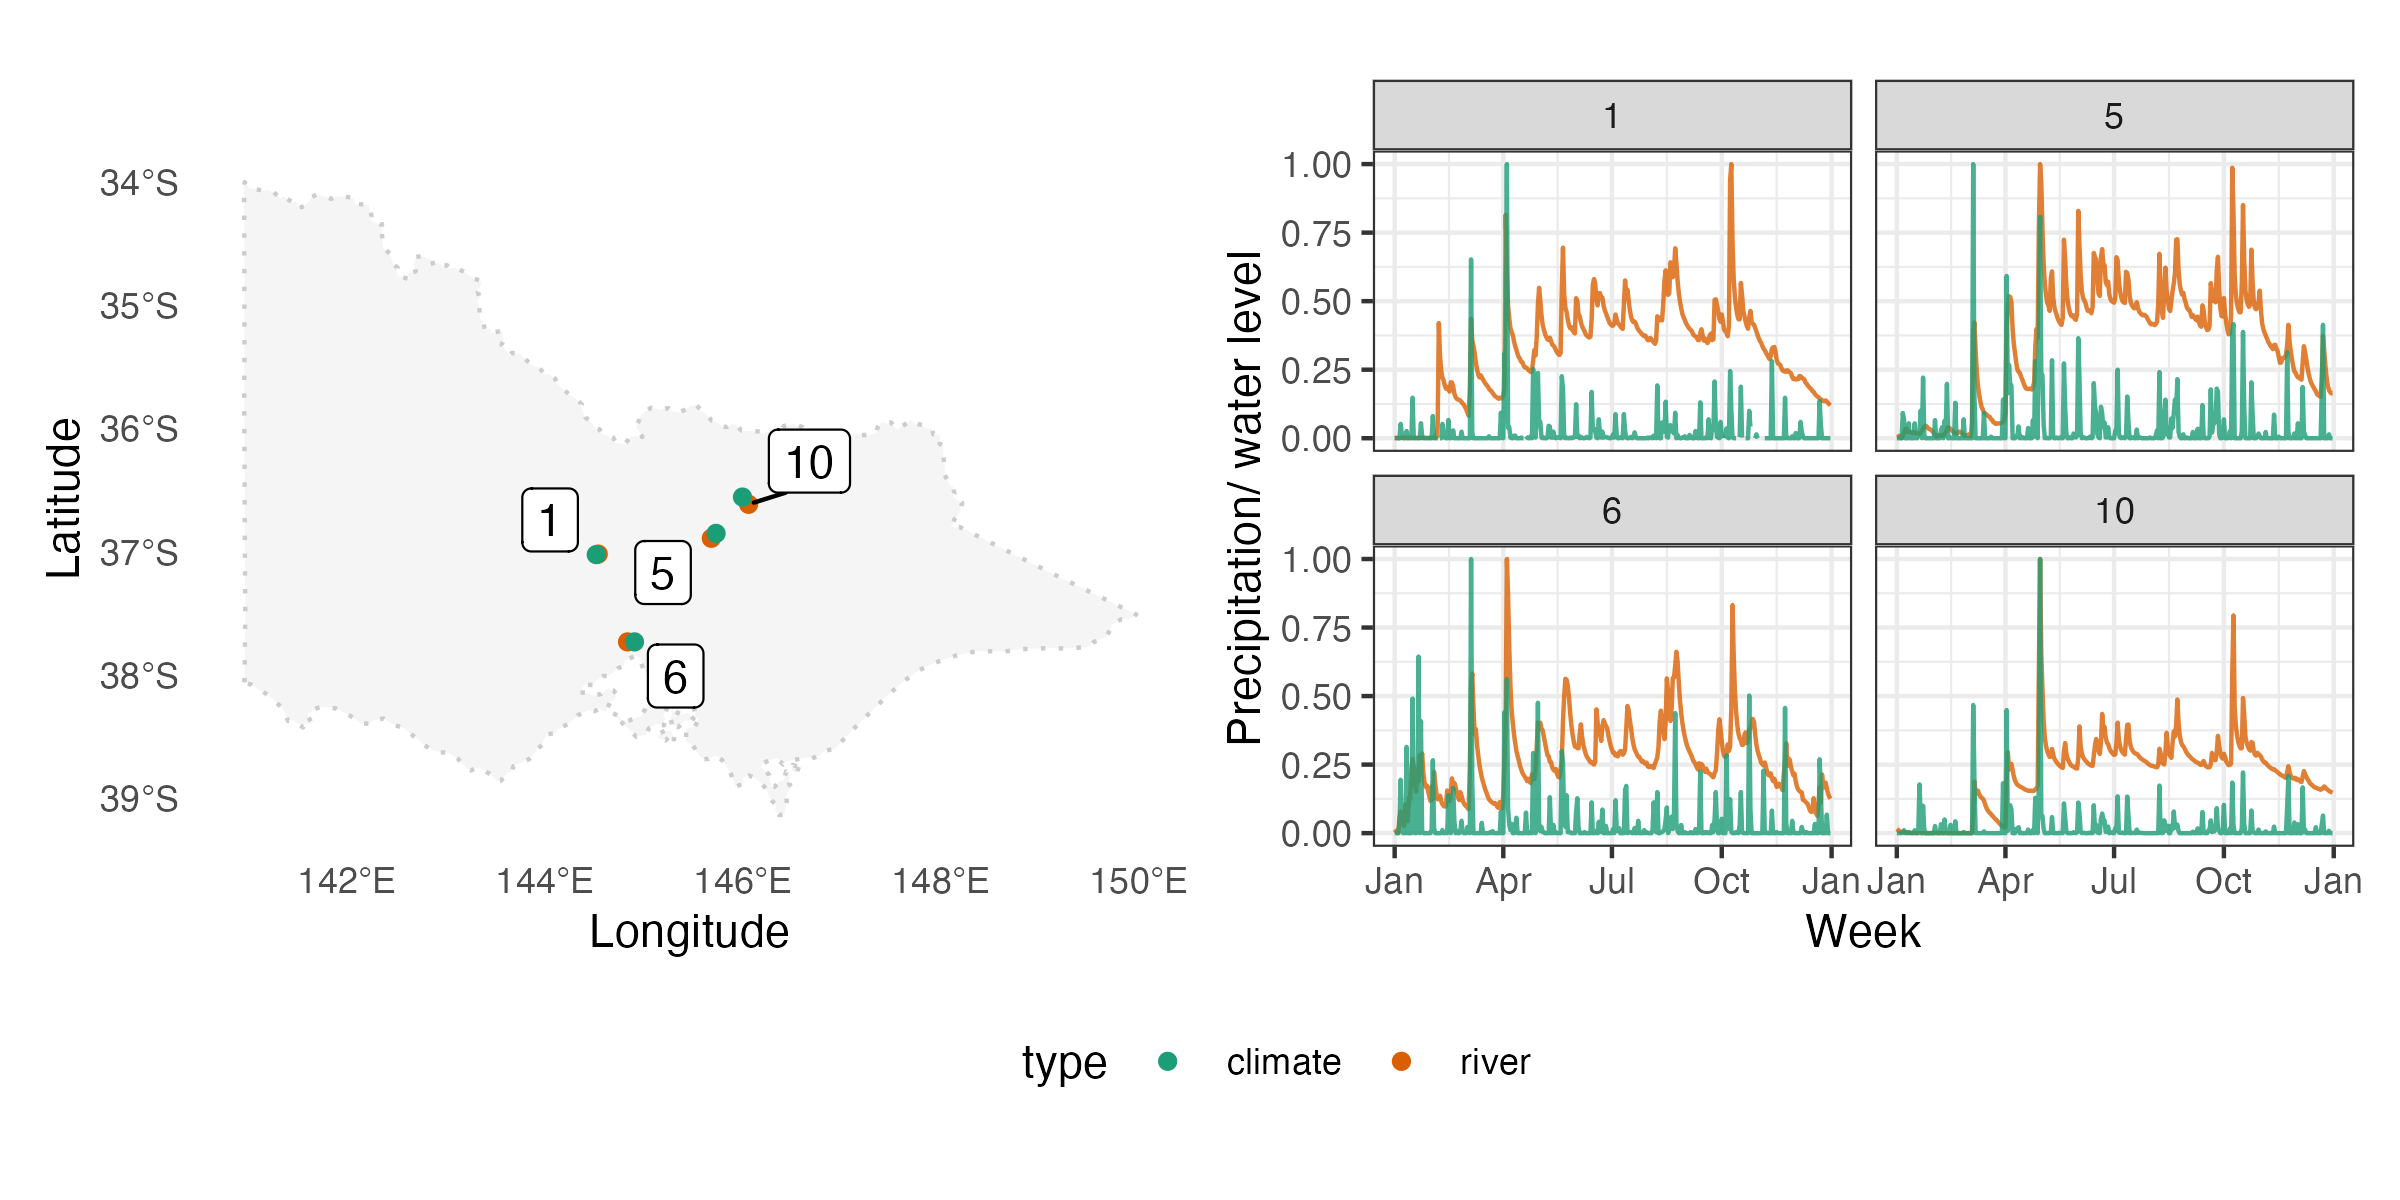
\includegraphics[width=1\linewidth]{figures/matching} 

}

\caption[Matched weather stations and river gauges on the map (A) and across time (B)]{Matched weather stations and river gauges on the map (A) and across time (B). Precipitation and water level have been standardised between 0 and 1 to be displayed on the same scale. The increases in the precipitation is reflected by the water level.}\label{fig:matching}
\end{figure}
\end{CodeChunk}

\hypertarget{era5-climate-reanalysis-data}{%
\subsection{ERA5: climate reanalysis
data}\label{era5-climate-reanalysis-data}}

ERA5 data \citep{hersbach2020era5} is the latest reanalysis of global
atmosphere, land surface, and ocean waves from 1950 onwards and is
available in the NetCDF format from European Centre for Medium-Range
Weather Forecasts (ECMWF). The data can be directly downloaded from
\href{https://cds.climate.copernicus.eu/cdsapp\#!/dataset/reanalysis-era5-pressure-levels?tab=overview}{Copernicus
Climate Data Store (CDS)} website or programmatically via an R package
\pkg{ecmwfr} \citep{ecwmfr}. The \code{era5-pressure} data contains
variable \emph{specific humidity} and \emph{geopotential} on the 10 hPa
pressure level on four dates: 2002-09-22, 2002-09-26, 2002-09-30, and
2002-10-04. Once downloaded, the data can be read into a cubble as:

\begin{CodeChunk}
\begin{CodeInput}
R> raw <- ncdf4::nc_open(here::here("data/era5-pressure.nc"))
R> dt <- as_cubble(raw, vars = c("q", "z"))
\end{CodeInput}
\end{CodeChunk}

Figure \ref{fig:netcdf} reproduces the ERA5 data row of Figure 19 in
\citet{hersbach2020era5}. It shows the southern polar vortex splits into
two on 2002-09-26 and further splits into four on 2002-10-04 in the
stratosphere. Readers interested in the analysis of this figure can
refer to \citet{hersbach2020era5}, \citet{simmons2020global} and
\citet{simmons2005ecmwf} for more details.

\begin{CodeChunk}
\begin{figure}

{\centering 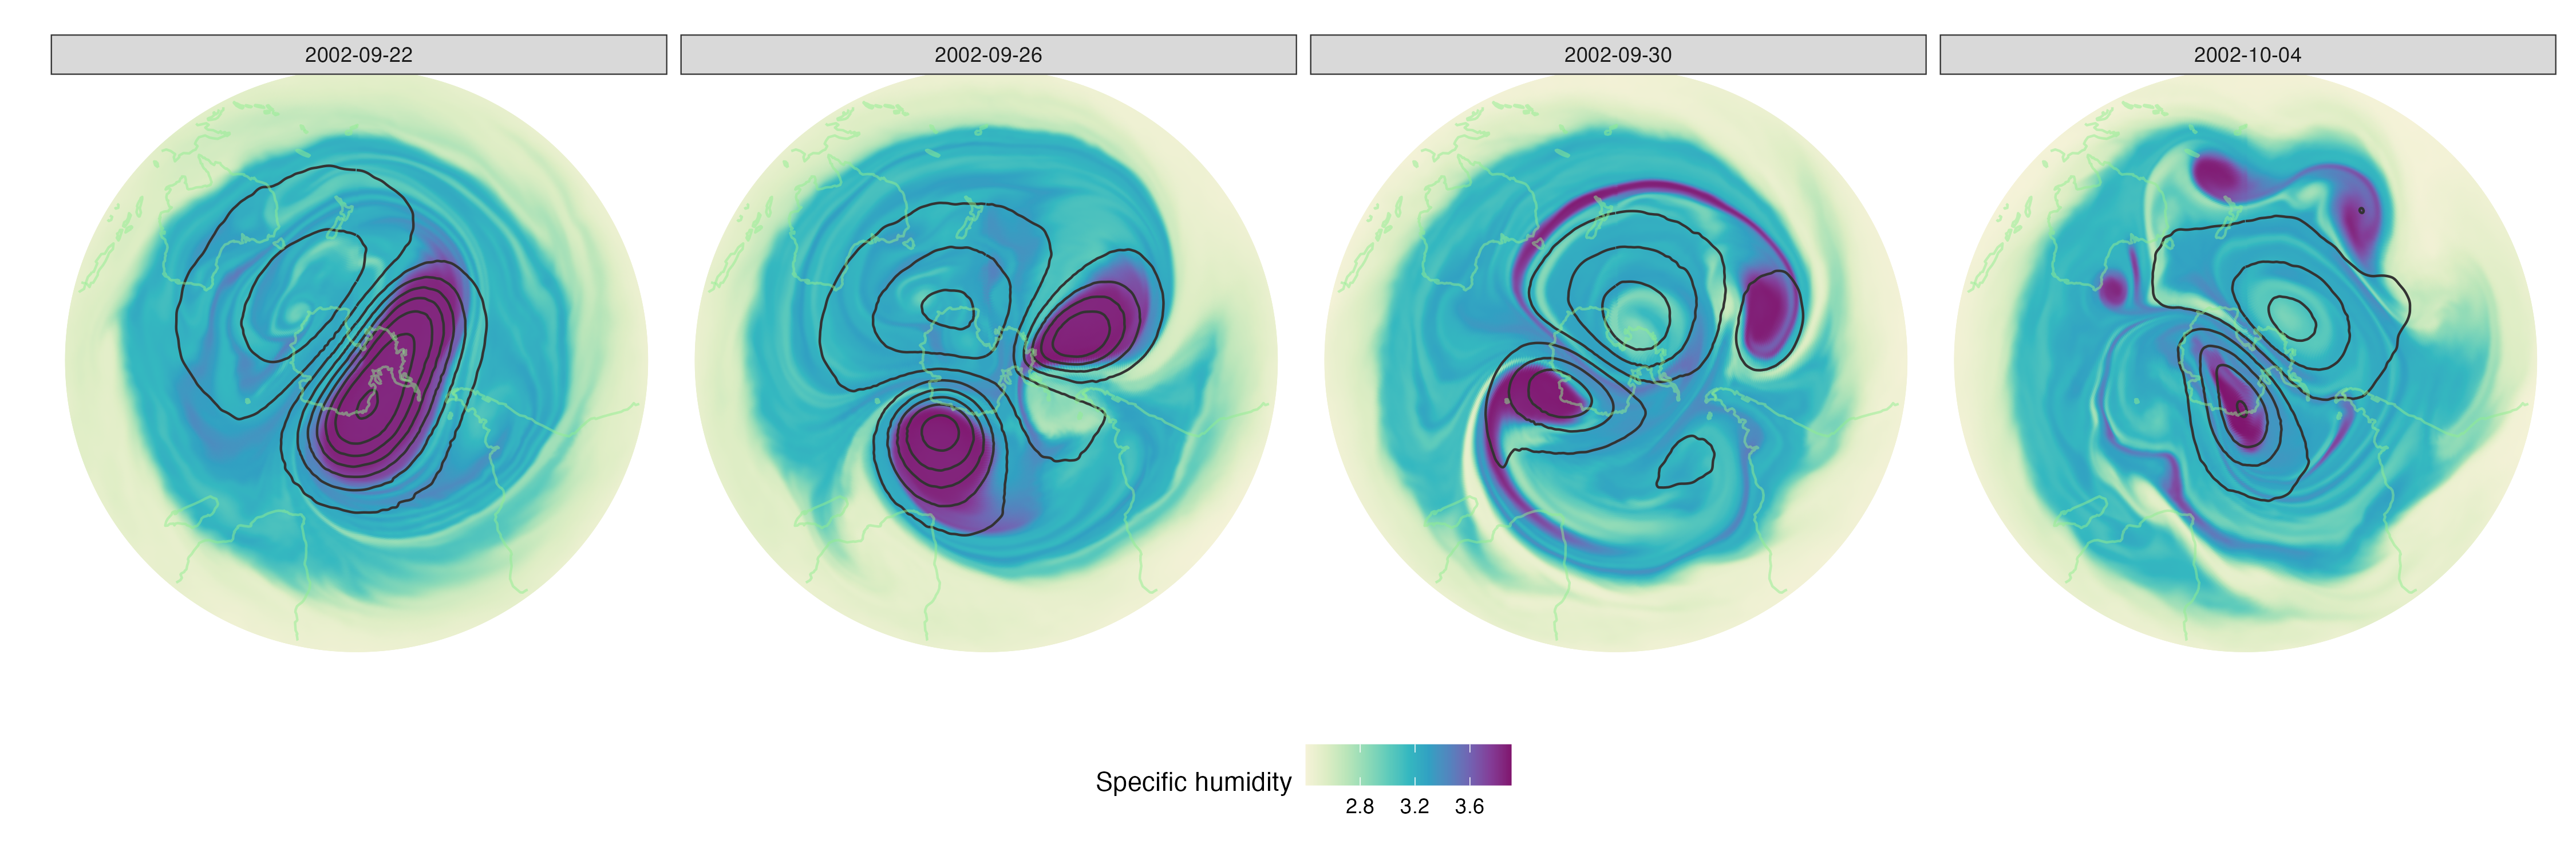
\includegraphics[width=1\linewidth]{/Users/sherryzhang/Documents/research/paper-cubble/figures/netcdf} 

}

\caption[A reproduction of the second row (ERA5 data) of Figure 19 in  Hersbach et al (2020)]{A reproduction of the second row (ERA5 data) of Figure 19 in  Hersbach et al (2020).}\label{fig:netcdf}
\end{figure}
\end{CodeChunk}

\hypertarget{interative-graphic-with-cubble}{%
\subsection{Interative graphic with
cubble}\label{interative-graphic-with-cubble}}

With spatio-temporal data, users may wish to make plots to learn the
spatial distribution of a variable, or to find patterns, such as trend
or seasonality, in the time series. Combining this two types of plot
with interactivity let users to link between points on the map and the
corresponding time series to explore the spatial and temporal dimension
of the data simultaneously. Below is an example that describes the
process of building an interactive graphic with \pkg{cubble} and
\pkg{crosstalk} The example explores the variation of monthly
temperature range with \code{weatherdata::climate_full} data.

The temperature range is calculated as the difference between
\code{tmax} and \code{tmin} and its monthly average over 2016 - 2020 is
taken before calculating the variance. A \code{SharedData} object is
constructed for each form of the cubble and the same \code{group}
argument ensures the cross-linking of the two forms via the common
\code{id} column. The spatial map and time series plot are then made
with each \code{SharedData} objects separately. In this example,
stations on the Australia map, made from the nested form, are coloured
by the calculated variance and a ribbon band is constructed using the
long form cubble to show the maximum and minimum temperature of each
station across month. With a different dataset, users are free to
calculate any per station measure in the nested form or to make any
time-wise summary of the data in the long form to customise the spatial
or temporal view. The cross-linking between the two plots is always
safeguarded by the shared \code{id} column embedded in the cubble
structure. Below is the pseudo code that outlines the process to
construct an interactive graphic described above:

\begin{CodeChunk}
\begin{CodeInput}
R> # data pre-processing
R> clean <- weatherdata::climate_full %>% ...
R> 
R> # created SharedData instance for crosstalk
R> nested <- clean %>% SharedData$new(~id, group = "cubble")
R> long <- stretch(clean) %>% SharedData$new(~id, group = "cubble")
R> 
R> # create the spatial and temporal view each with a ShareData instance
R> p1 <- nested %>% ...
R> p2 <- long %>% ...
R> 
R> # Combine p1 and p2
R> crosstalk::bscols(plotly::ggplotly(p1), plotly::ggplotly(p2), ...)
\end{CodeInput}
\end{CodeChunk}

In Figure \ref{fig:interactive-linking}, the first row shows the initial
view of the interactive graphic. On the map, most regions in Australia
have low variance of temperature range while the north-west coastline,
bottom of South Australia, and Victoria stands out with larger monthly
changes. In the second row, Mount Elizabeth is selected on the map given
its high variance colour on the initial map and this links to the ribbon
on the right. The third row the lowest temperature in August and this
corresponds to Thredbo AWS in the Victoria and New South Wales border.
Another station in the Tasmania island is selected on the map to cross
compare with Thredbo AWS.

\begin{CodeChunk}
\begin{figure}

{\centering 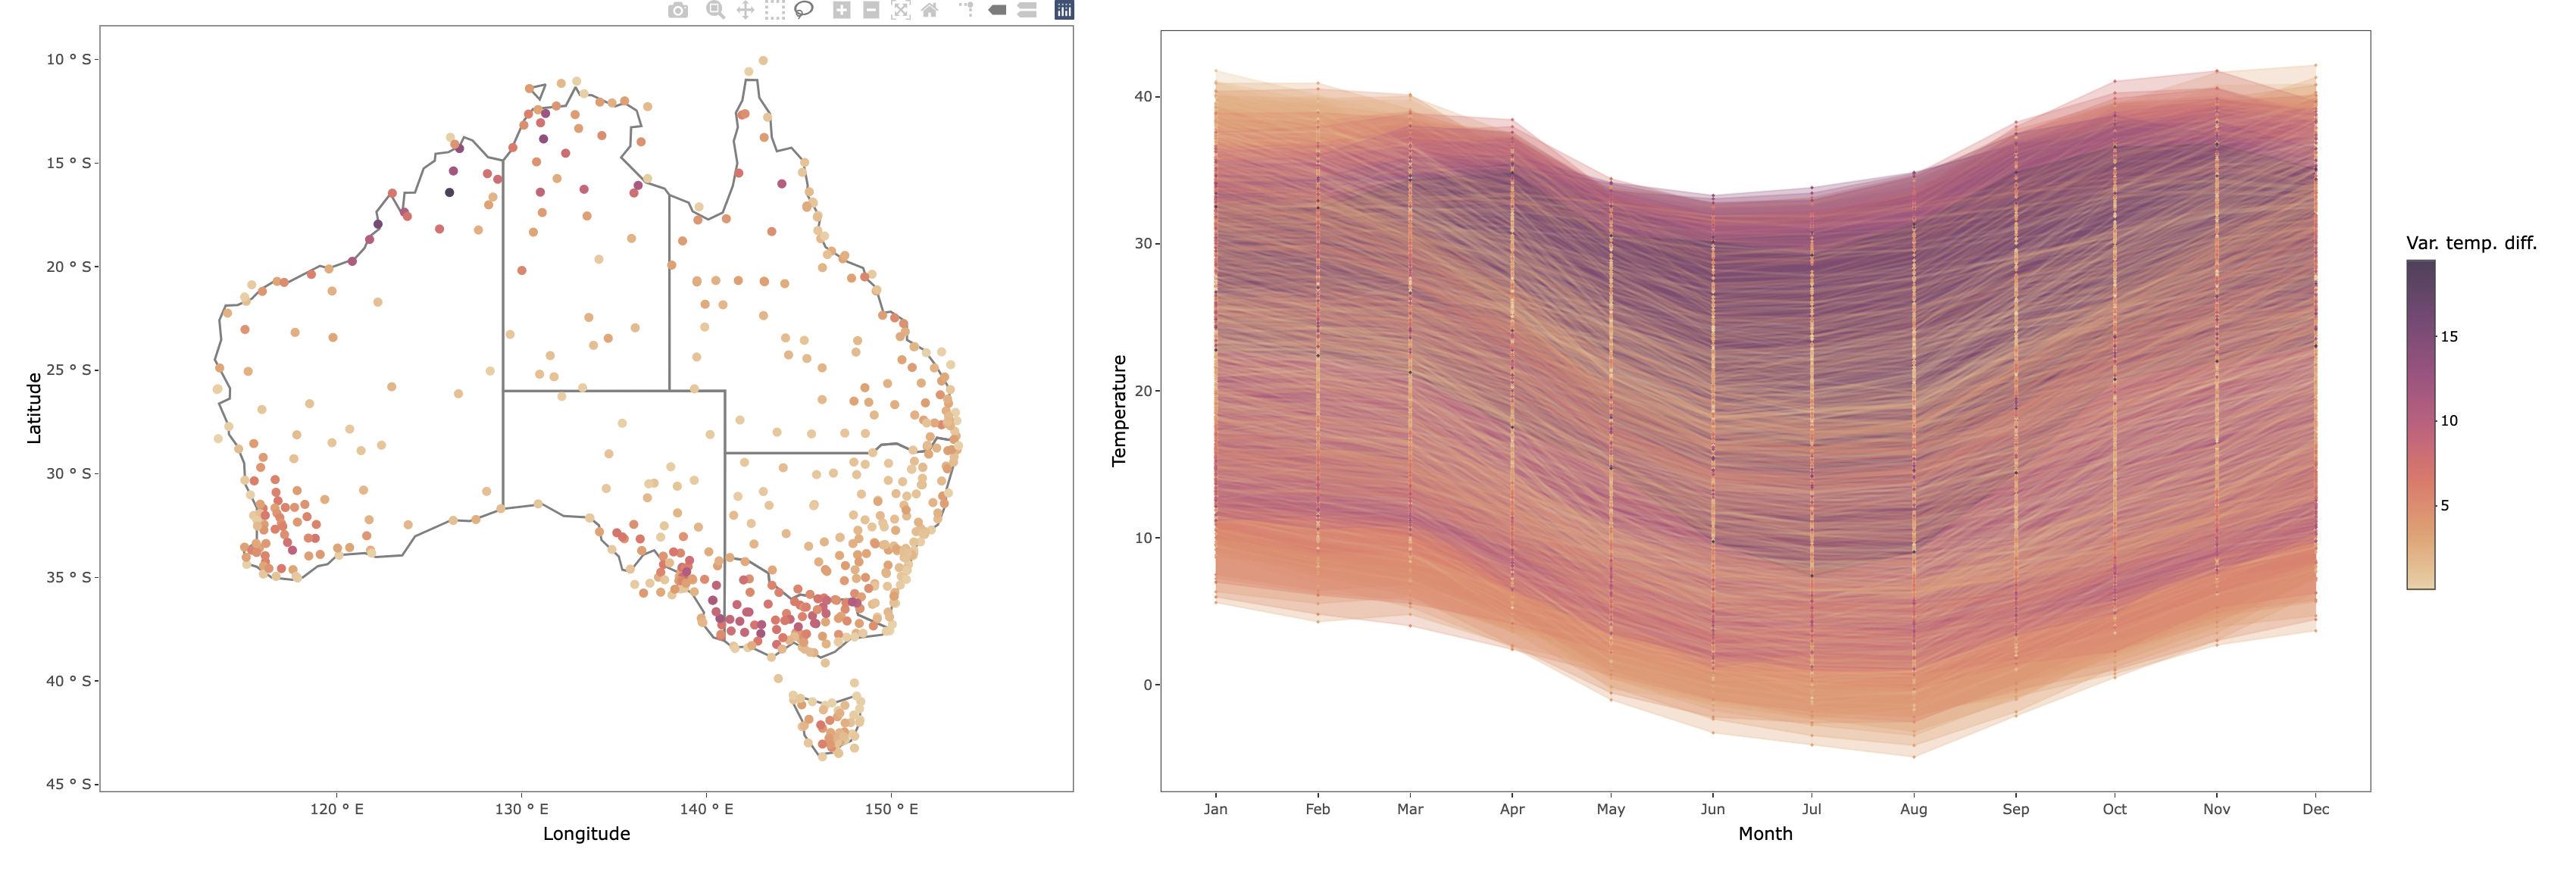
\includegraphics[width=1\linewidth,height=0.23\textheight]{/Users/sherryzhang/Documents/research/paper-cubble/figures/linking} 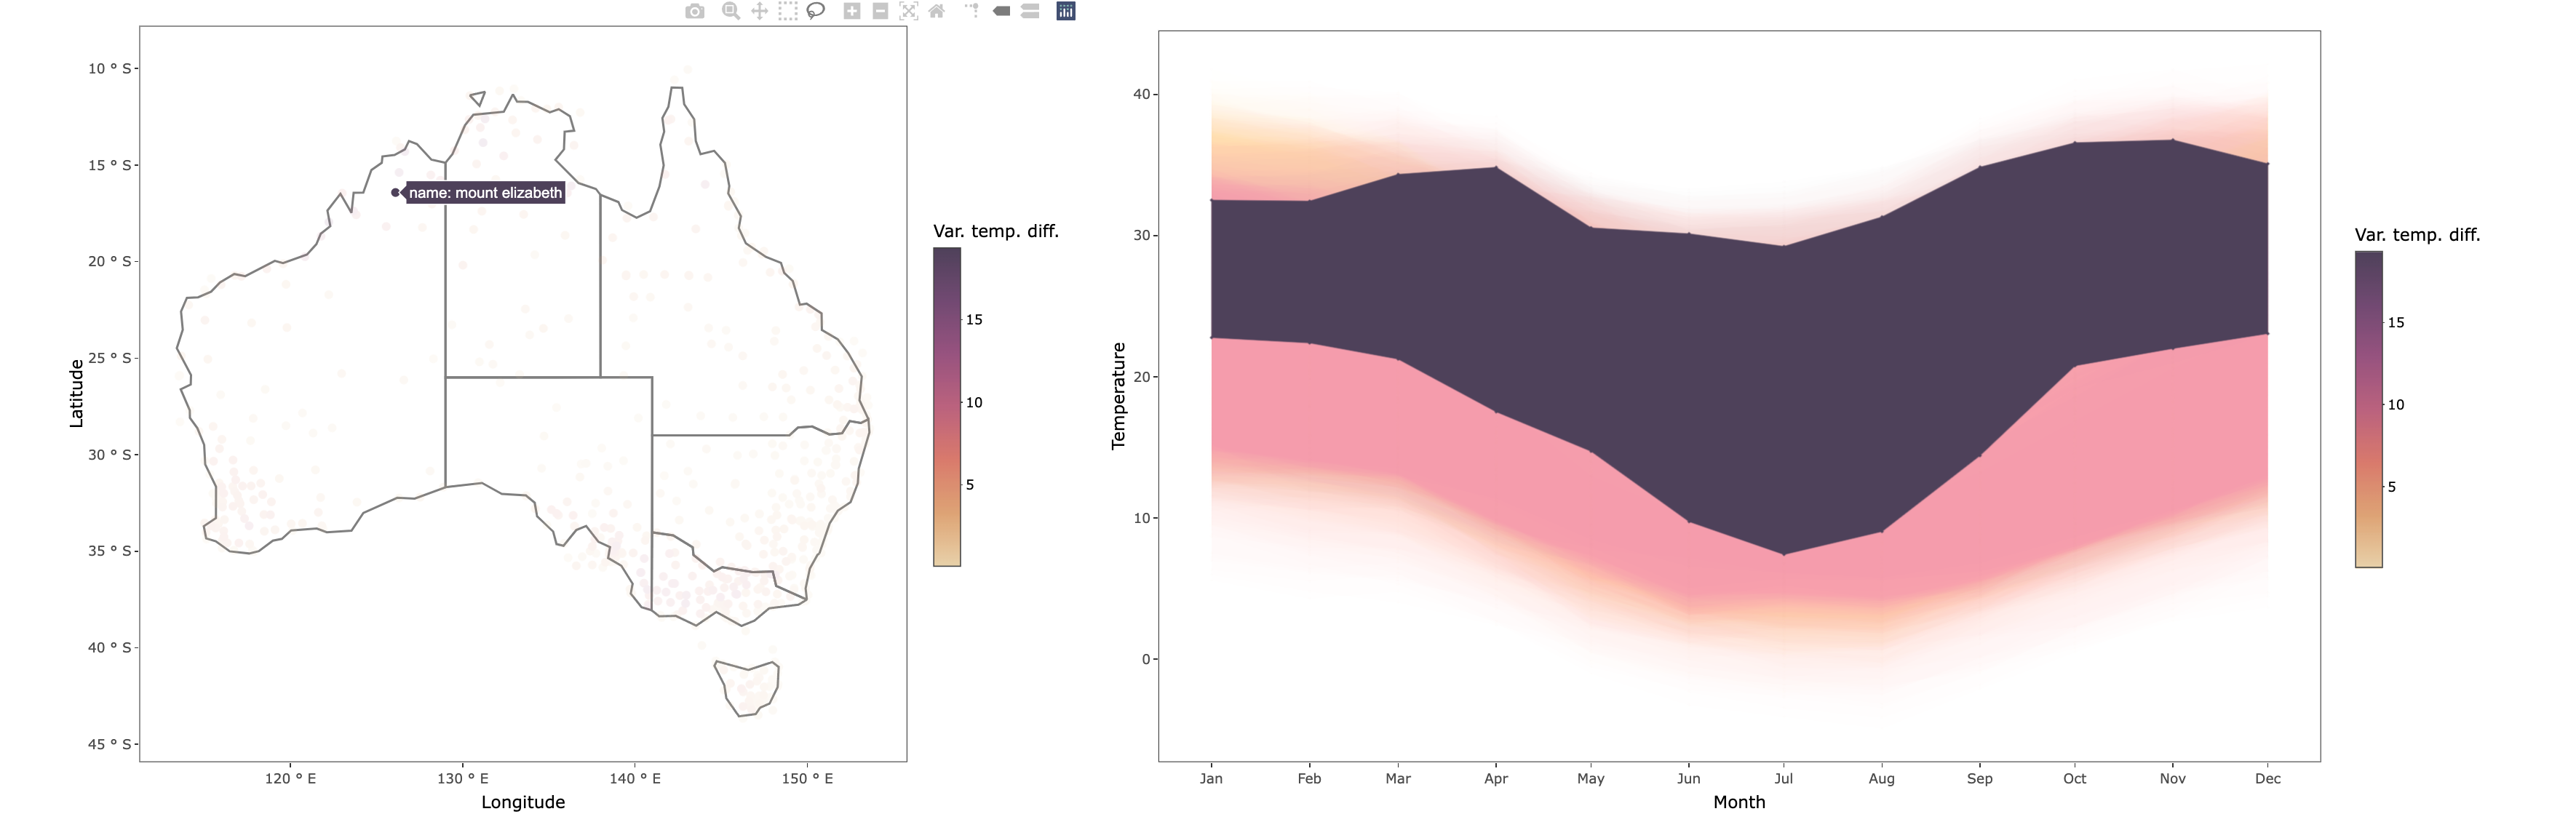
\includegraphics[width=1\linewidth,height=0.23\textheight]{/Users/sherryzhang/Documents/research/paper-cubble/figures/linking-north} 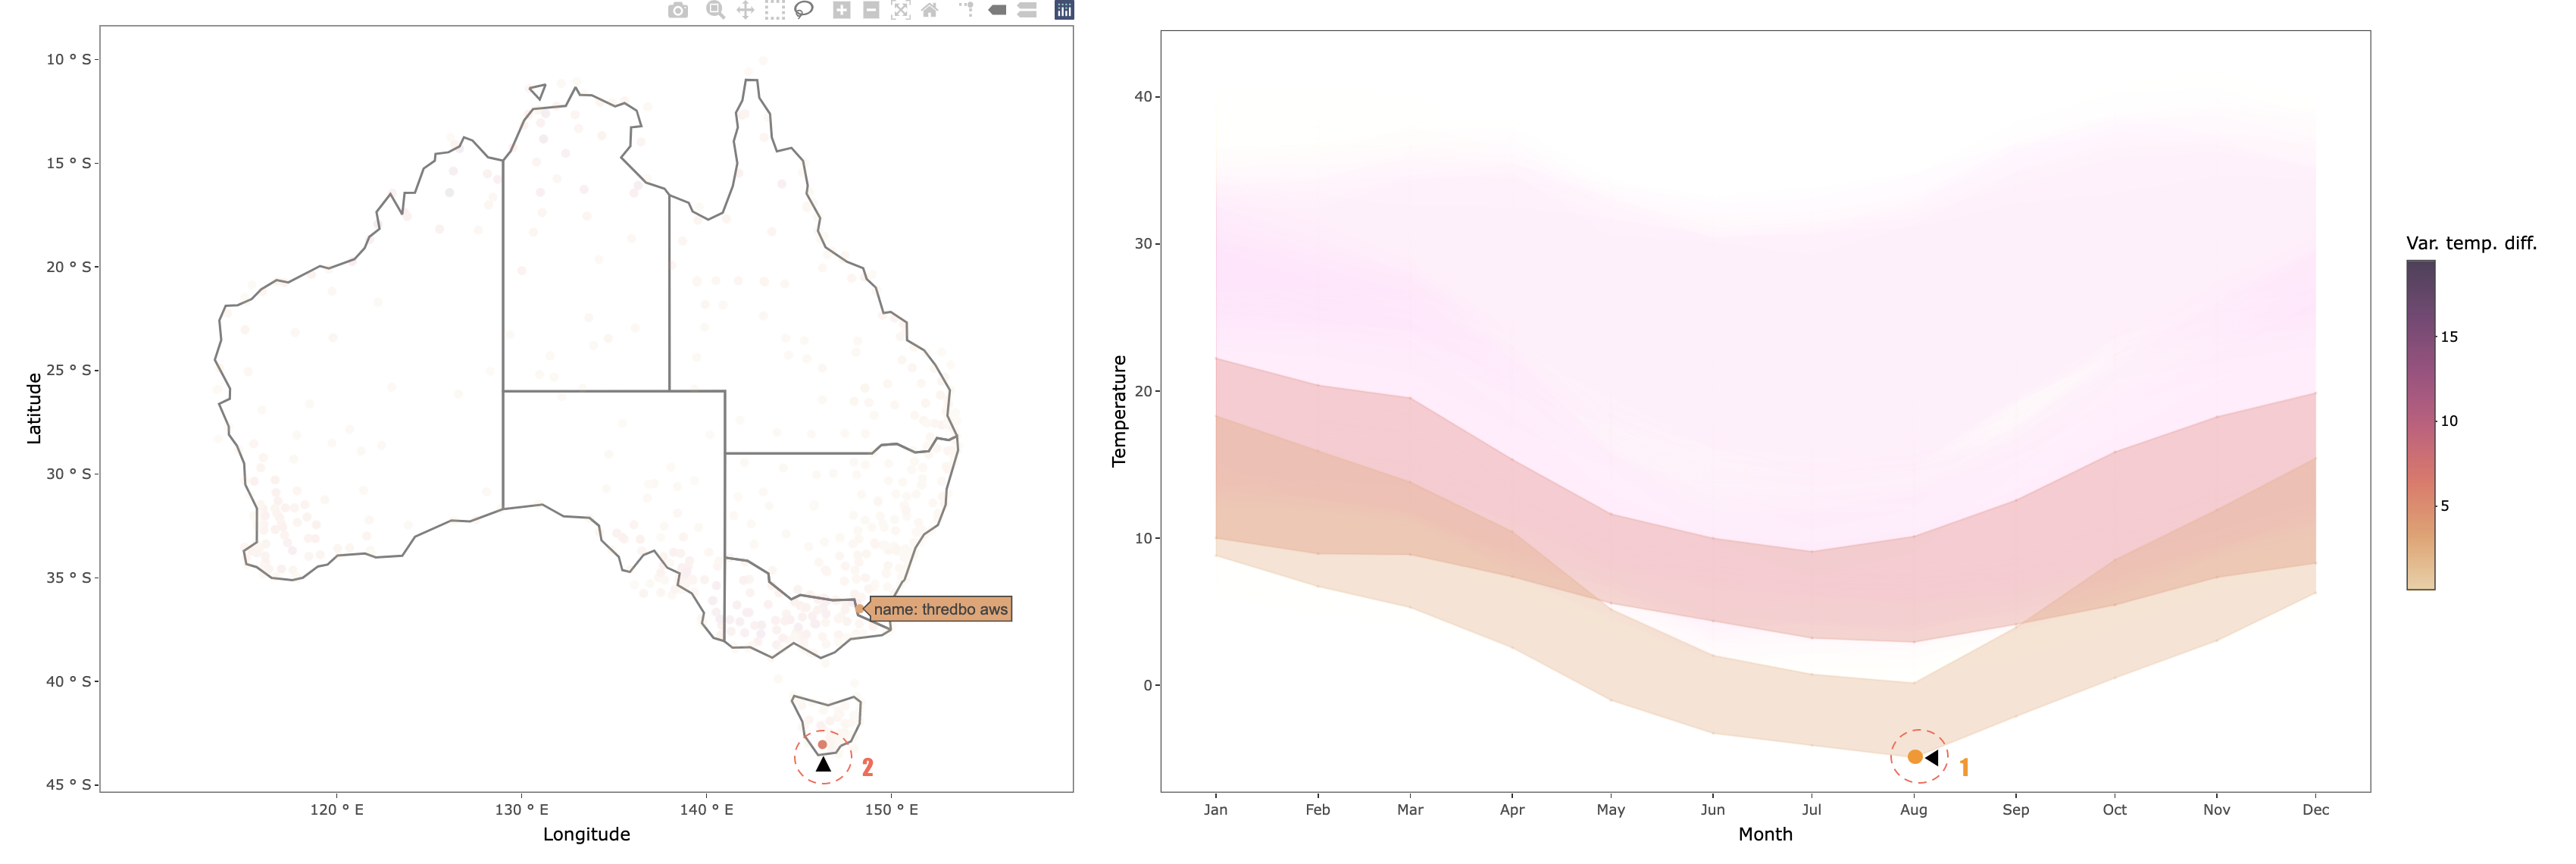
\includegraphics[width=1\linewidth,height=0.23\textheight]{/Users/sherryzhang/Documents/research/paper-cubble/figures/linking-lower} 

}

\caption[Exploring temperature variation using linking of a map and seasonal display]{Exploring temperature variation using linking of a map and seasonal display. Each row is a screen dump of the process. The top row shows all locations and all temperature profiles. Selecting a location with high variance on the map produces the plot in the second row. The maximum nad minimum temperature is shown using a ribbon. The bottom row first selects the lowest temperature in Auguest in the seasonal display. A location in the Tasmania Island is then selected to compare the temperature variation with Thredbo AWS.}\label{fig:interactive-linking}
\end{figure}
\end{CodeChunk}

This plot can also be made using \pkg{cubble} and \pkg{leaflet} where
the temperature range can be displayed as a small subplot upon clicking
on the map. This would require first creating the popup plots from the
long form cubble as a vector and then add these plots to a leaflet map
created from the nested cubble, with \code{leafpop::addPopupGraphs()}:

\begin{CodeChunk}
\begin{CodeInput}
R> # data pre-processing
R> clean <- weatherdata::climate_full %>% ...
R> 
R> # use the long form to create subplots for each station
R> df_id <- unique(clean$id)
R> p <- map(1:length(df_id), function(i){
+   dt <- clean %>% filter(id == df_id[i])
+   ggplot(dt) %>% ...
+ })
R> 
R> # create nested form leaflet map with temperature band as subplots 
R> nested <- tamp(clean)
R> leaflet(nested) %>% 
+   addTiles() %>% 
+   addCircleMarkers(group = "a", ...) %>% 
+   leafpop::addPopupGraphs(graph = p, ...)
\end{CodeInput}
\end{CodeChunk}

Figure \ref{fig:interactive-popup} shows Figure
\ref{fig:interactive-linking} made made with leaflet and popups
\citep{leafpop}.

\begin{CodeChunk}
\begin{figure}

{\centering 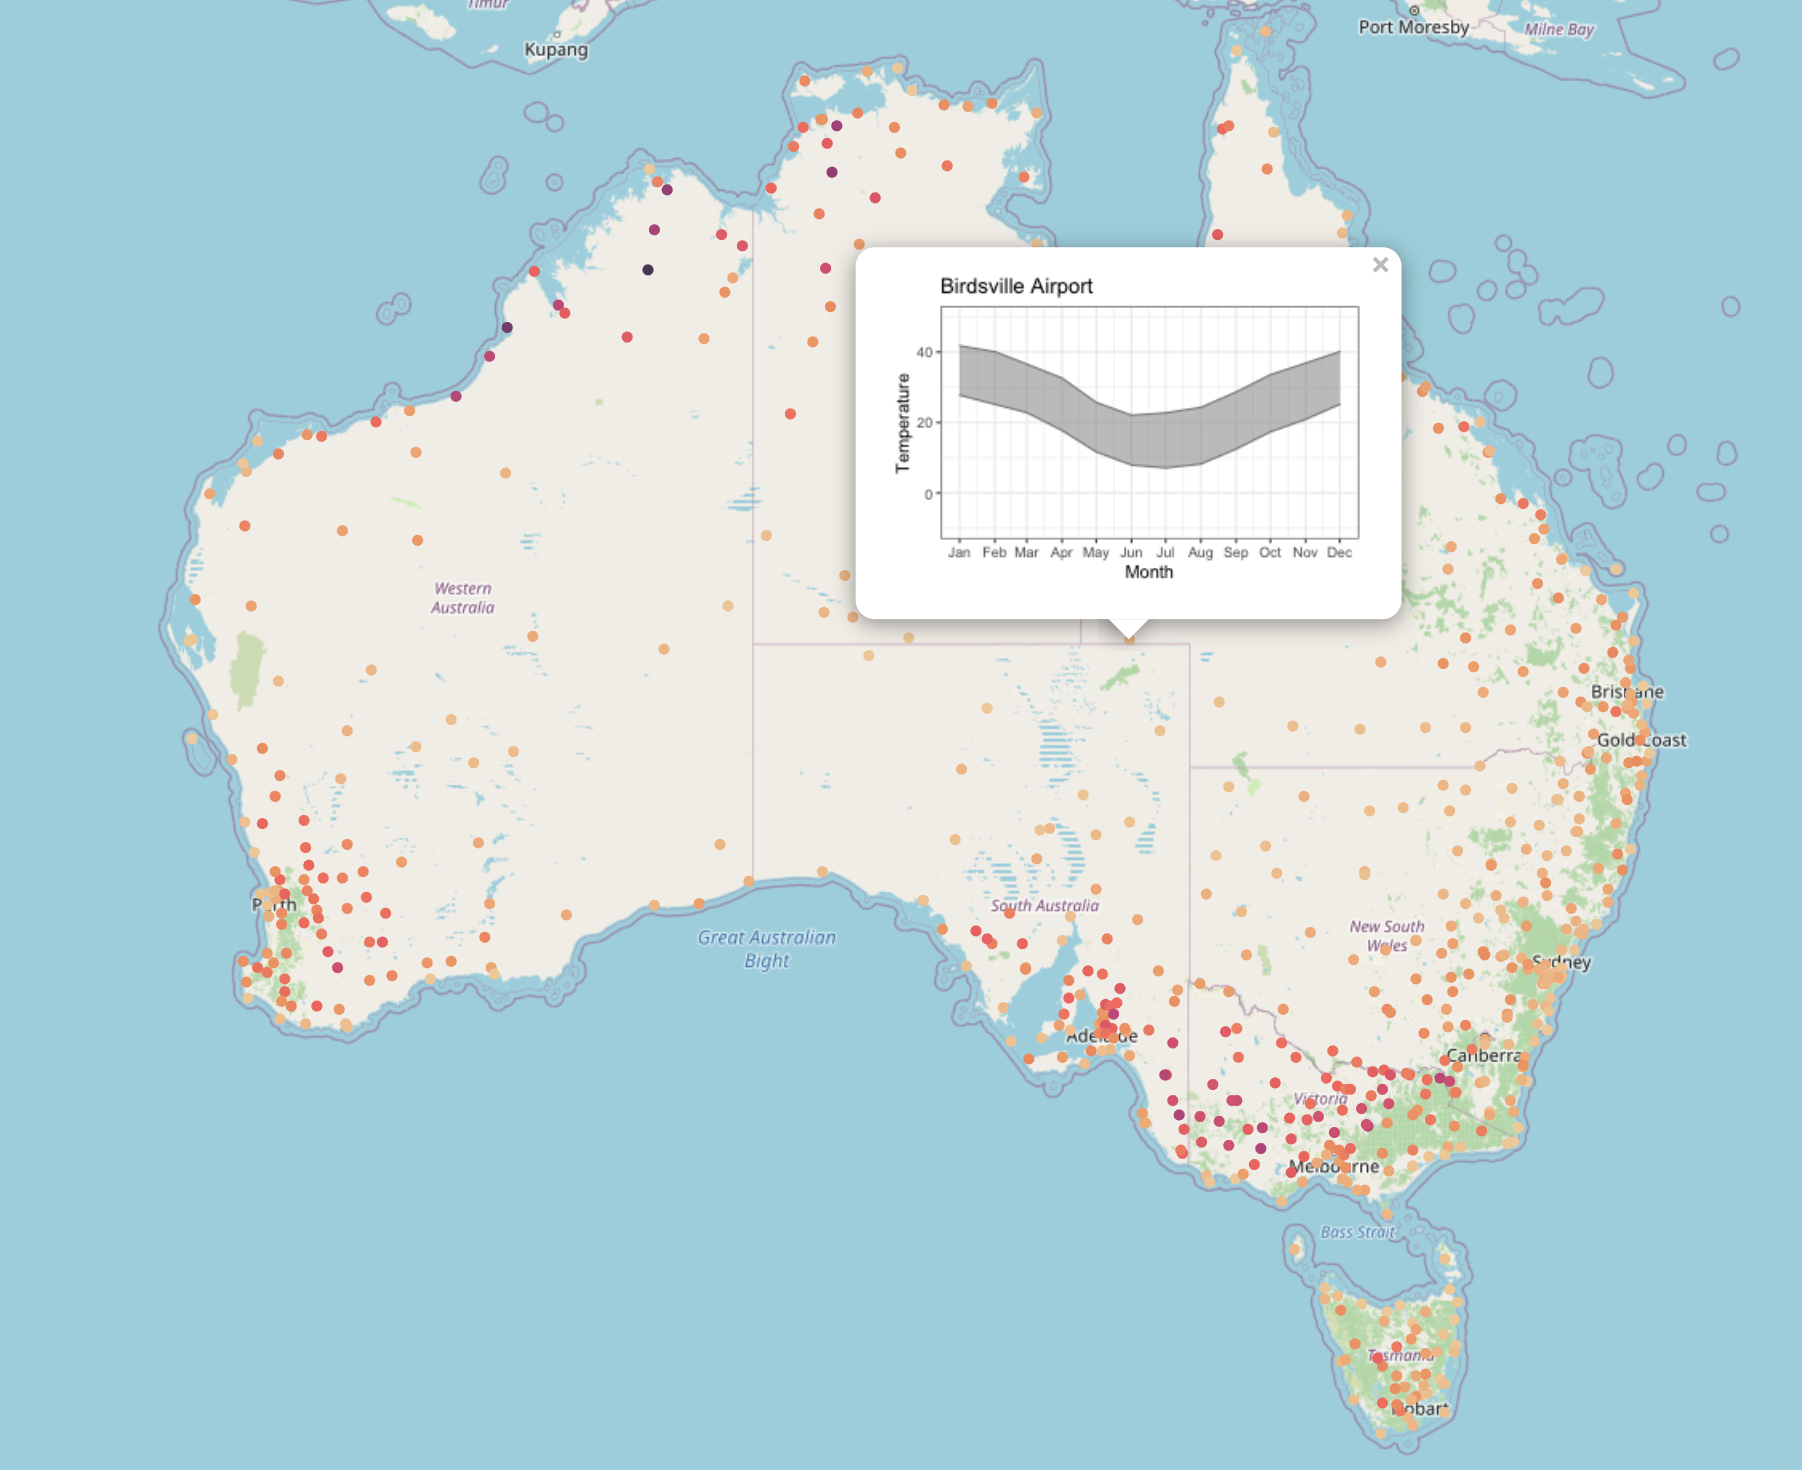
\includegraphics[width=0.45\linewidth,height=0.25\textheight]{/Users/sherryzhang/Documents/research/paper-cubble/figures/popup-mid} 

}

\caption[Same as Figure 11 with thetemperature variation shown as a popup in the leaflet map]{Same as Figure 11 with thetemperature variation shown as a popup in the leaflet map.}\label{fig:interactive-popup}
\end{figure}
\end{CodeChunk}

\hypertarget{conclusion}{%
\section{Conclusion}\label{conclusion}}

This paper describes an \proglang{R} package \pkg{cubble} for
manipulating and visualising spatio-temporal data. A new data structure,
\code{cubble} that builds from the \code{rowwise_df} and
\code{grouped_df} class in the tidyverse ecosystem, is proposed to
connect the time invariant and varying variables in the spatio-temporal
data. This design frees the data analysts from spending time on
organising variables of different observational units. The data
structure is also flexible to the techniques and packages analysts use
to analyse the data, for example, in the matching example in section
4.3, users are free to use algorithms from another package to cluster
stations.

Further development and maintenance of the package involves responding
to changes in the tidyverse packages that \pkg{cubble} imports, in
particular, \pkg{tibble}, \pkg{tidyr}, and \pkg{dplyr}. Another area for
further development is to extend \pkg{cubble} to other spatial objects
other than points.

\newpage

\hypertarget{acknowledgement}{%
\section{Acknowledgement}\label{acknowledgement}}

This work is funded by the Commonwealth Scientific and Industrial
Research Organisation (CSIRO) Data61 Scholarship and started while
Nicolas Langrené was affiliated with CSIRO's Data61. The article is
created using \pkg{knitr} \citep{knitr} and \pkg{rmarkdown}
\citep{rmarkdown} in R. The source code for reproducing this paper can
be found at: \url{https://github.com/huizezhang-sherry/paper-cubble}.

\hypertarget{appendix}{%
\section{Appendix}\label{appendix}}

\begin{CodeChunk}
\begin{figure}

{\centering 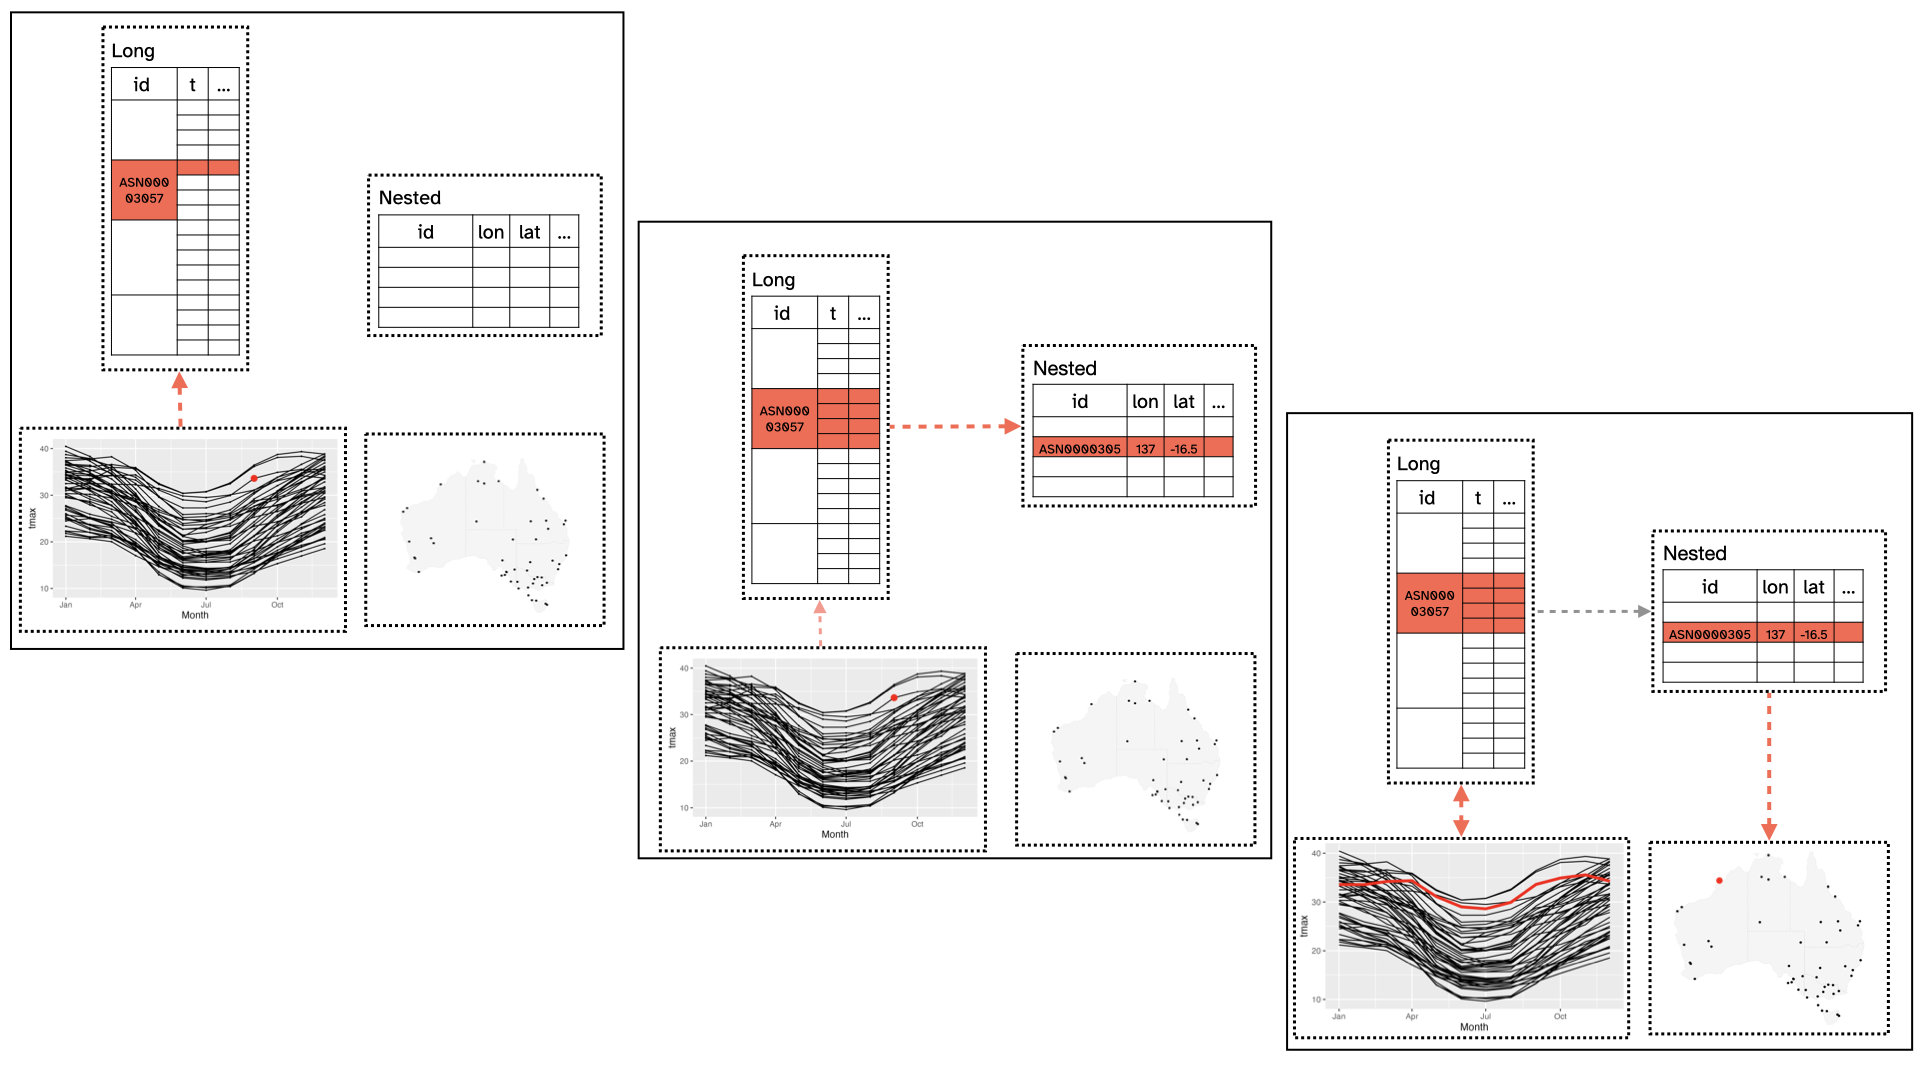
\includegraphics[width=1\linewidth,height=0.4\textheight]{/Users/sherryzhang/Documents/research/paper-cubble/figures/diagram-keynotes/diagram-keynotes.005} 

}

\caption[An illustration of the data model under interactive graphics with cubble]{An illustration of the data model under interactive graphics with cubble. When a point on the time series is selected, the corresponding row in the long cubble will be activated. This will link to all the rows with the same id in the long cubble and the row in the nested cubble with the smae id (middle). Both plots will be updated with the full line selected and the point highlighted on the map (right).}\label{fig:illu-interactive-2}
\end{figure}
\end{CodeChunk}

\newpage

\bibliography{references.bib}


\end{document}
